\documentclass{report}
\usepackage{graphicx}
\usepackage{braket}
\usepackage[italian]{babel}
\usepackage{float}
\usepackage{wrapfig}
\usepackage{amsmath}
\usepackage{amssymb}
\usepackage{braket}
\usepackage{parskip}
\usepackage{cancel}
\usepackage{bbold}
\usepackage{upgreek}
\usepackage{hyperref}
\usepackage{caption}
\usepackage{tikz}
\usepackage{mathtools}
\DeclarePairedDelimiter{\ceil}{\lceil}{\rceil}

\usepackage{geometry}
\renewcommand{\figurename}{Figura}
\geometry{
	a4paper,
	total = {160mm,260mm},
	left = 21mm,
	top = 18mm,
}


\title{\textbf{\Huge Quantum Information}\\ {\Large \textbf{\textit{Appunti del corso}}}}
\author{\textit{Giuseppe Scordo,} \\ \textit{Stefano Mavilla,} \\ \textit{Damiano Trovato}}
\date{Anno Accademico 2025/26}

\begin{document}

\maketitle
\tableofcontents

\chapter*{Introduzione al Corso}

Quantum information è un corso sulla teoria dell'informazione che si compone di 2 parti
\begin{itemize}
	\item 3 CFU di Introduzione alla \textbf{Teoria dell'Informazione Classica}
	\item 3 CFU di Introduzione alla \textbf{Teoria dell'Informazione Quantistica}
\end{itemize}
Cos'è la Teoria dell'Informazione?\\
Fino a che punto possiamo comprimere i dati?\\
Qual'è il miglior tasso di trasmissione possibile?
\begin{itemize}
	\item \textbf{Teoria classica dell'informazione}
	\\ Ci chiediamo cosa sia l'informazione e come renderla affidabile su canali inaffidabili. Vediamo in breve cenni di teoria dell'informazione di Shannon:
	\begin{itemize}
		\item È possibile inviare informazione con probabilità di errore $\varepsilon$, se il tasso di comunicazione è minore della capacità del canale
		\item Ogni segnale ha complessità intrinseca (\textit{entropia}) oltre al quale non può essere compreso
		\item Se l'entropia della sorgente è minore della capacità di canale, una comunicazione (asintoticamente) priva di errori può avvenire
	\end{itemize}
	\item  \textbf{Teoria dell'informazione quantistica}
	\\A differenza del caso precedente utilizziamo i qubit. Quello che fa davvero la differenza sono i \textit{termini di coerenza}, usando le matrici di densità. 
	Un'altra differenza è la presenza dell'\textbf{entanglement}.
	Studieremo come misurare l'entropia di uno stato quantistico (Entropia di Von Neumann).
\end{itemize}
Vedremo le seguenti misure: Capacità classica, quantistica e quantistica assistita (con entanglement).

\part{Teoria dell'Informazione Classica}
\chapter{Prima comunicazione su canale rumoroso}

\section{Come possiamo garantire una comunicazione perfetta in un canale imperfetto e rumoroso?}
Nella trasmissione di informazione, come stringhe di bit, in un canale di comunicazione imperfetto, esiste una probabilità che al ricevente del messaggio \textbf{non arrivi lo stesso messaggio} inviato dal mittente.

Esempi di canali di comunicazione variano dai cavi di una linea telefonica analogica ai dischi rigidi di un moderno PC, fino alle cellule riproduttive.

\section{Canale Binario Simmetrico}
Nel modello di comunicazione conosciuto come \textbf{Canale Binario Simmetrico} viene trasmesso dal mittente una stringa di bit.

\begin{minipage}{0.60\textwidth}
	Ogni bit $x$ che verrà trasmesso al ricevente può essere corrotto con probabilità $f$ (con 0 $\leq f \leq 1$) o arrivare correttamente con probabilità $1-f$.\\ Indichiamo inoltre ogni bit ricevuto come $y$.
\end{minipage}
\begin{minipage}{0.45\textwidth}
	\begin{figure}[H]
		\centering
		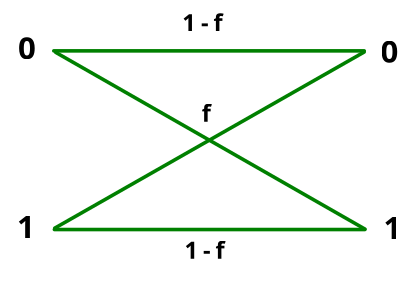
\includegraphics[width=0.5\textwidth]{images/Canale.png}
	\end{figure}
\end{minipage}

$$
P(y = 0|x= 0) = 1 -f;\quad P(y = 0| x=1) = f;
$$
$$
P(y=1|x=0) = f;\quad P(y=1|x=1) = 1 - f;
$$


\subsection{Soluzioni alla corruzione di bit in un canale di comunicazione}
Esistono in letteratura due approcci per mitigare la creazione di errori in un canale di comunicazione, la soluzione \textbf{fisica} e quella \textbf{logica}.

\textbf{Soluzione fisica}

La soluzione fisica consiste nel migliorare le caratteristiche fisiche del canale per ridurne la probabilità di errore. Tipicamente le modifiche ad un'infrastruttura fisica ne aumentano i costi.

\textbf{Soluzione sistemica}

La Teoria dell'Informazione e la Teoria dei Codici offrono un approccio diverso. Accettando di comunicare in un canale rumoroso, possiamo \textbf{trovare} e \textbf{correggere} gli errori introdotti da quest'ultimo.

Aggiungendo un \textit{encoder} prima del canale, possiamo codificare il \textbf{messaggio sorgente} $s$ nel messaggio \textbf{trasmesso} $t$, aggiungendo ad esso della \textbf{ridondanza}.\\ Il canale \textbf{corrode} il messaggio $t$ in un messaggio $r$ che, arrivato alla fine del canale, verrà decodificato da un \textit{decoder}, che userà la ridondanza per ricostruire il messaggio $s$.

\newpage
\begin{figure}[h]
	\centering
	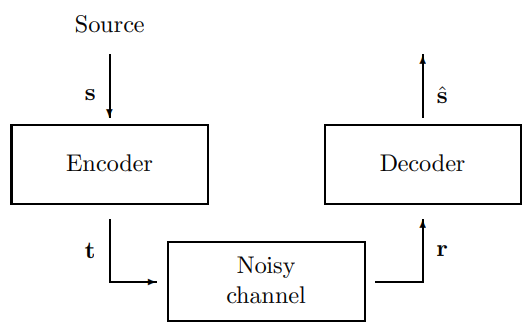
\includegraphics[width=0.5\textwidth]{images/encoder_decoder.png}
\end{figure}

Ma come possiamo aggiungere ridondanza ad un messaggio? E come possiamo \textbf{trovare} e \textbf{correggere} errori in un messaggio?

\section{Tecniche di Correzione degli errori in un Canale Binario Simmetrico}

Prima di addentrarci sulle tecniche di Error-Correction in un canale di comunicazione, è importante definire il \textbf{Tasso di Trasmissione}, ovvero:

\begin{center}
	\textit{Il rapporto tra i bit che vogliamo inviare e quelli effettivamente codificati}.
\end{center}

\subsection{Codici di Ripetizione}
Un'idea semplice per aggiungere ridondanza consiste nel \textbf{ripetere ogni bit} del messaggio $s$ per $n$ volte. Scegliendo $n$ dispari, il decoder correggerà il messaggio $r$ scegliendo il bit che compare più frequentemente in ogni sequenza di $n$ bit.

Ad esempio, se ripetessimo ogni bit 3 volte, avremmo una codifica $R_3$, quindi per ogni 3 bit sceglieremmo quello che compare almeno 2 volte.

\textbf{Esempio di Error-Correction con Codici di Ripetizione}

Immaginiamo di voler trasmettere il messaggio $s$: \verb|0110| e ipotizziamo che $f = 0.1$.\\Allora con probabilità $1-f=0.9$ il bit sarà corretto.

Utilizziamo una codifica $R_3$ per codificare il messaggio $s$ nel messaggio $t$:
$$
0 \rightarrow 000 \hspace{1cm} 1 \rightarrow 111\hspace{1cm} 1 \rightarrow 111 \hspace{1cm}0 \rightarrow 000
$$
Supponiamo che nel canale il messaggio $t$ sia stato corrotto nel messaggio $r$:
$$
010 \rightarrow 0 \hspace{1cm} 101 \rightarrow 1\hspace{1cm} 111 \rightarrow 1 \hspace{1cm}100 \rightarrow 0
$$
Nell'esempio fatto, questo semplice algoritmo ha corretto $r$ nel messaggio $s$ originale. Tuttavia i \textbf{Codici di Ripetizione} presentano due grossi limiti:
\begin{enumerate}
	\item Un Tasso di Trasmissione \textbf{molto basso}, in quanto con una codifica $R_n$, il bitrate è di soli $\frac{1}{n}$ bit.
	\item Con una cattiva distribuzione degli errori, l'algoritmo potrebbe non riuscire a correggere correttamente $r$, decodificando un $s'\neq s$. Si potrebbe aumentare la ridondanza per evitare questo scenario, ma la prima limitazione avrebbe ancora più effetto. 
\end{enumerate}

La \textbf{probabilità} di ottenere una decodifica $s'\neq s$ in una codifica $R_3$ diventa: 
$$P[E_3] = \sum^{3}_{i=2} \binom{3}{i} f^i(1-f)^{3-i}=\binom{3}{2}f^2(1-f)+f^3 = 3f^2-2f^3=O(f^2)$$
con $0\leq f \leq1$, quindi $f^2 > f^3$.

Se volessimo ridurre la probabilità di ottenere una decodifica $s'\neq s$ potremmo passare ad una codifica $R_5$. Notiamo che questa funzione vale per questo specifico canale \textbf{senza perdita} di bit.

\newpage
In $R_5$ abbiamo un tasso di pardita:
$$
P[E_5]=\sum^{5}_{i=3} \binom{5}{i}f^i(1-f)^{5-i} = \binom{5}{3} f^3(1-f)^2 + \binom{5}{4} f^4(1-f) + f^5
$$
$$
P[E_5]= 10f^3 (1-f)^2 + 5f^4(1-f) + f^5 = O(f^3)
$$

Se volessimo fare lo stesso calcolo per una decodifica $R_N$ avremmo:
$$
P[E_N]=\sum^{N}_{i=\frac{N+1}{2}} \binom{N}{i}f^i(1-f)^{N-i} = O(f^{\frac{N+1}{2}})
$$
Notiamo che la \textbf{crescita è lineare} e che dovremmo usare troppo spazio per tassi d'errore tendenti allo zero.

\textbf{Variazione con doppia codifica}

Supponiamo di codificare la stessa stringa $s$ nella codifica $R_9$. Calcolando la probabilità di ottenere una decodifica $s\neq s'$ otterremmo $P[E_9]=O(f^6)$.

Sfruttando una variante dei Codici di Ripetizione con una doppia codifica, codificando $R_9$ come $R^2_3$, cioè codificando due volte in $R_3$.\\ 
Come esempio prendiamo il messaggio $s$: \verb|1101| che con questa codifica diventa:
$$
1 \rightarrow 111 \qquad 1 \rightarrow 111 \qquad 0 \rightarrow 000 \qquad 1 \rightarrow 111 \qquad
$$
e successivamente:
$$
111 \rightarrow 111111111 \qquad 111 \rightarrow 111111111 \qquad 000 \rightarrow 000000000 \qquad 111 \rightarrow 111111111 \qquad
$$

Otteniamo: 
$$
P[E_{R^2_3}]=\sum^{3}_{i=2}\binom{3}{i}P^i_{2R_3}(1-P_{2R_3})^{3-i} \approx O(f^4)
$$
che risulta \textbf{peggiore} dell'algoritmo classico, quindi paghiamo lo spazio con l'errore.


\subsection{Codici a Blocco - Hamming (7,4)}
Possiamo ottenere trasmettere messaggi $s$ con una bassa probabilità di errore e con un tasso di trasmissione accettabile? Si, tramite i codici a \textbf{Blocchi}.

Un codice a blocco è una \textbf{regola} per convertire una sequenza di bit sorgente $s$ di lunghezza $K$ in una sequenza $t$ di lunghezza $N$, con $N > K$. Gli extra bit $N-K$ sono funzioni lineari degli originali $K$ bit e sono chiamati \textbf{bit di parità}.

Un esempio di codice a blocco lineare è il Codice di Hamming (7,4) che trasmette $N=7$ bit per ogni $K=4$ bit sorgente.
I quattro bit di informazione che vogliamo trasmettere sono indicati come $s_1, s_2, s_3, s_4$ mentre i bit di parità sono indicati con $t_1, t_2, t_3$, scelti affinché:

\begin{minipage}{0.50\textwidth}
	\begin{center}
		\begin{tikzpicture}[scale=0.4]
			\tikzstyle{every node}+=[inner sep=0pt]
			\draw [black] (35.7,-21.3) circle (3);
			\draw (35.1,-21.5) node {$t_3$};
			\draw [black] (37.9,-18.1) circle (3);
			\draw (37.9,-17.5) node {$t_1$};
			\draw [black] (39.9,-21.3) circle (3);
			\draw (40.5,-21.5) node {$t_2$};
			\draw (39.3,-19.7) node {$s_2$};
			\draw (36.4,-19.7) node {$s_1$};
			\draw (37.9,-22) node {$s_4$};
			\draw (37.9,-20.3) node {$s_3$};
		\end{tikzpicture}
	\end{center}
\end{minipage}
\begin{minipage}{0.45\textwidth}
	$$s_1+s_2+s_3+t_1=0 \mod2$$
	$$s_2+s_3+s_4+t_2=0 \mod2$$
	$$s_1+s_3+s_4+t_3=0 \mod2$$
\end{minipage}

Il tasso di trasmissione è $\frac{4}{7}$, \textbf{migliore} rispetto a quello dei Codici di Ripezione.
\newpage
\subsubsection{Esempio di Error-Correction con Hamming (7,4)}

Trasmettiamo nuovamente il messaggio $s$: \verb|1101|. Calcolando i bit di parità, otteniamo:

\begin{minipage}{0.50\textwidth}
	\begin{center}
		\begin{tikzpicture}[scale=0.4]
			\tikzstyle{every node}+=[inner sep=0pt]
			\draw [black] (35.7,-21.3) circle (3);
			\draw (35.1,-21.5) node {$t_3$};
			\draw [black] (37.9,-18.1) circle (3);
			\draw (37.9,-17.5) node {$t_1$};
			\draw [black] (39.9,-21.3) circle (3);
			\draw (40.5,-21.5) node {$t_2$};
			\draw (39.3,-19.7) node {$1$};
			\draw (36.4,-19.7) node {$1$};
			\draw (37.9,-22) node {$1$};
			\draw (37.9,-20.3) node {$0$};
		\end{tikzpicture}
	\end{center}
\end{minipage}
$\Rightarrow$
\begin{minipage}{0.50\textwidth}
	\begin{center}
		\begin{tikzpicture}[scale=0.4]
			\tikzstyle{every node}+=[inner sep=0pt]
			\draw [black] (35.7,-21.3) circle (3);
			\draw (35.1,-21.5) node {$0$};
			\draw [black] (37.9,-18.1) circle (3);
			\draw (37.9,-17.5) node {$0$};
			\draw [black] (39.9,-21.3) circle (3);
			\draw (40.5,-21.5) node {$0$};
			\draw (39.3,-19.7) node {$1$};
			\draw (36.4,-19.7) node {$1$};
			\draw (37.9,-22) node {$1$};
			\draw (37.9,-20.3) node {$0$};
		\end{tikzpicture}
	\end{center}	
\end{minipage}

Supponiamo che adesso il secondo bit del messaggio $t$ venga corrotto durante la trasmissione nel canale e che diventi il messaggio $r$: \verb|1001000|. Una volta che arriva al decoder, quest'ultimo è in grado di \textbf{individuare e correggere l'errore}, in quanto rileva una somma dispari.

\begin{minipage}{0.50\textwidth}
	\begin{center}
		\begin{tikzpicture}[scale=0.4]
			\tikzstyle{every node}+=[inner sep=0pt]
			\draw [black] (35.7,-21.3) circle (3);
			\draw (35.1,-21.5) node {$0$};
			\draw [black] (37.9,-18.1) circle (3);
			\draw (37.9,-17.5) node {$0$};
			\draw [black] (39.9,-21.3) circle (3);
			\draw (40.5,-21.5) node {$0$};
			\draw (39.3,-19.7) node {$0^*$};
			\draw (36.4,-19.7) node {$1$};
			\draw (37.9,-22) node {$1$};
			\draw (37.9,-20.3) node {$0$};
		\end{tikzpicture}
	\end{center}	
\end{minipage}
$\Rightarrow$
\begin{minipage}{0.50\textwidth}
	\begin{center}
		\begin{tikzpicture}[scale=0.4]
			\tikzstyle{every node}+=[inner sep=0pt]
			\draw [black] (35.7,-21.3) circle (3);
			\draw (35.1,-21.5) node {$0$};
			\draw [black] (37.9,-18.1) circle (3);
			\draw (37.9,-17.5) node {$0$};
			\draw [black] (39.9,-21.3) circle (3);
			\draw (40.5,-21.5) node {$0$};
			\draw (39.3,-19.7) node {$1^*$};
			\draw (36.4,-19.7) node {$1$};
			\draw (37.9,-22) node {$1$};
			\draw (37.9,-20.3) node {$0$};
		\end{tikzpicture}
	\end{center}	
\end{minipage}

\subsubsection{Sindrome della decodifica dei Codici di Hamming}
Supponiamo ancora una volta di voler trasmettere il messaggio $s$: \verb|1101| che viene codificato nel messaggio $t$: \verb|1101000|.
Questa volta tuttavia si corrompono i bit $s_2$ ed $s_3$ e al decoder arriva il messaggio $r$: \verb|1011000|.

\begin{center}
	\begin{tikzpicture}[scale=0.4]
		\tikzstyle{every node}+=[inner sep=0pt]
		\draw [black] (35.7,-21.3) circle (3);
		\draw (35.1,-21.5) node {$0$};
		\draw [black] (37.9,-18.1) circle (3);
		\draw (37.9,-17.5) node {$0$};
		\draw [black] (39.9,-21.3) circle (3);
		\draw (40.5,-21.5) node {$0$};
		\draw (39.3,-19.7) node {$0^*$};
		\draw (36.4,-19.7) node {$1$};
		\draw (37.9,-22) node {$1$};
		\draw (37.9,-20.3) node {$1^*$};
	\end{tikzpicture}
\end{center}	

Il decoder procederà al rilevamento e alla correzione degli errori. Il risultato della decodifica è il seguente messaggio $s'$: \verb|1011001|, diverso da $s$.

\begin{center}
	\begin{tikzpicture}[scale=0.4]
		\tikzstyle{every node}+=[inner sep=0pt]
		\draw [black] (35.7,-21.3) circle (3);
		\draw (35.1,-21.5) node {$1*$};
		\draw [black] (37.9,-18.1) circle (3);
		\draw (37.9,-17.5) node {$0$};
		\draw [black] (39.9,-21.3) circle (3);
		\draw (40.5,-21.5) node {$0$};
		\draw (39.3,-19.7) node {$0^*$};
		\draw (36.4,-19.7) node {$1$};
		\draw (37.9,-22) node {$1$};
		\draw (37.9,-20.3) node {$1^*$};
	\end{tikzpicture}
\end{center}

Ebbene, i codici di Hamming (7,4) \textbf{falliscono} nella correzione di messaggi con \textbf{almeno due errori}.\\  Sia $E_H$ l'evento che i bit vengano inviati con errori. Allora la probabilità di averne 2 è:
$$
P[E_H]=\sum^{7}_{i=2}\binom{7}{i}f^i(1-f)^{7-i}=O(f^2)
$$
uguale a quella della codifica $R_3$, ma con un tasso di trasmissione molto più elevato.

Se vogliamo un tasso d'errore alto sembrerebbe che anche il bitrate debba esserlo. Shannon ci dice che possiamo avere un tasso d'errore basso e un bitrate consistentemente diverso da 0.

\chapter{Fondamenti di probabilità}

\section{Variabili aleatorie}
Una \textbf{variabile aleatoria} (V.A.) è una tripla ($x$, $A_x$, $P_x$), dove il risultato $x$ è il valore di una variabile casuale di un insieme di possibili valori $A_x=\{a_0,a_1,\cdots,a_{n-1}\}$, ognuno con probabilità $P_x=\{p_0, p_1,\cdots,p_{n-1}\}$.
%
Sulla probabilità, valgono i seguenti assiomi:
\begin{enumerate}
	\item \textbf{Non negatività}: Dato un evento $E$ allora $P(E) \ge0$
	\item \textbf{Additività}: Siano $A,B$ 2 V.A. indipendenti, allora $P[A\cup B]=P[A]+P[B]$
	\item \textbf{Normalizzazione}: Sia $E$ l'evento certo, $P[E]=1 $
\end{enumerate}

Da questi assiomi possiamo dimostrare tutti i teoremi sulle probabilità. Possiamo ad esempio dimostrare la probabilità dell'evento impossibile $I$.
$$P[E] = P[E\cup I]=P[E]+P[I]=1+P[I]\Rightarrow P[I] = P[E]-1 = 0$$
Da ora in poi useremo la notazione: $P[A,B] = P[A\cap B] = P[A\wedge B]$

\subsection{Teoremi su Variabili Aleatorie}
Date 2 variabili aleatorie $X,Y$ con supporti $A_x,A_y$ valgono i seguenti teoremi:
\begin{itemize}
	\item \textbf{Teorema della Probabilità Totale}: $$
	P[X=x_i]=\sum_{y\in A_y}P[X=x_i \wedge Y = y_i]$$
	\item \textbf{Probabilità Marginale}: Possiamo ottenere $P(x)$ da $P(x,y)$ tramite una sommatoria: 
	$$
	P(x=a_i) \equiv \sum_{y\in A_Y} P(x=a_i, y) \quad \Rightarrow \quad P(y) = \sum_{x\in A_X} P(x,y)
	$$
	\item \textbf{Probabilità condizionata}: $$P[X|Y]=\frac{P[X\wedge Y]}{P[Y]}$$
	da cui segue: $$P[X=x\wedge Y =y]=P[X=x|Y=y]P[Y=y]$$
	\item \textbf{Teorema di Bayes}: $$P[X|Y] = \frac{P[Y|X]P[X]}{P[Y]}$$
\end{itemize}

\subsubsection{Esempio N.1 - Meccanico}
Alice porta la sua auto dal meccanico. Il meccanico, Bob,
dopo aver effettuato un test computerizzato, sostiene che un pezzo molto costoso debba essere sostituito. Sia \textbf{a} la variabile aleatoria che indica lo stato effettivo del pezzo (a=1 il pezzo è guasto, a=0 il pezzo non è guasto). Si supponga di sapere inoltre che:
\begin{enumerate}
	\item Il test fatto da Bob ha un’affidabilità del 95\%. Nel 95\% dei casi in cui il pezzo è rotto allora la risposta fornita è “il pezzo è rotto”. Nel 95\% dei casi in cui il pezzo non è rotto allora la risposta fornita è “il pezzo non è rotto”;
	\item Solo l’1\% delle vetture (in condizioni analoghe a quella di Alice) ha avuto problemi con il pezzo in questione. 
\end{enumerate}
Qual è la probabilità che il pezzo sia effettivamente guasto?

Indichiamo con $a$ la variabile aleatoria che ci dà lo \textbf{stato effettivo del pezzo}:
\begin{enumerate}
	\item Con $a=1$ il pezzo \textbf{è} guasto, dove $Pr[a=1] = \frac{1}{100}$
	\item Con $a=0$ il pezzo \textbf{non è} guasto, dove $Pr[a=0] = \frac{99}{100}$
\end{enumerate}

e con $b$ la V.A. che ci dà \textbf{l'esito del test}:

\begin{enumerate}
	\item Con $b=1$ il test dice "Rotto".
	\item Con $b=0$ il test dice "OK".
\end{enumerate} 

Sappiamo inoltre che:
\begin{itemize}
	\item $P[b=1|a=1] = \frac{95}{100} \qquad \Rightarrow \qquad P[b=0|a=1] = \frac{5}{100}$
	\item $P[b=0|a=0] = \frac{95}{100} \qquad \Rightarrow \qquad P[b=1|a=0] = \frac{5}{100}$
\end{itemize}

Per trovare la probabilità che il pezzo sia effettivamente guasto dobbiamo trovare:
$$
P[a=1|b=1] =  \frac{P[a=1 \wedge b=1]}{P[b=1]} 
$$

Per prima cosa troviamo $P[a=1 \wedge b=1]$ che sappiamo è uguale a:
$$
P[b=1|a=1]\cdot P[a=1] = \frac{95}{100} \cdot \frac{1}{100}
$$

Successivamente troviamo $P[b=1]$ che sappiamo è uguale a:
$$
P[b=1 \wedge a=1] + P[b=1 \wedge a=0]
$$

Possiamo ricavare $P[b=1 \wedge a=0]$, essendo uguale a:
$$
P[b=1 | a=0] \cdot P[a=0] = \frac{5}{100} \cdot \frac{99}{100}
$$

Riscriviamo il tutto e ricaviamo $P[a=1|b=1]$:
$$
P[a=1|b=1] =  \frac{P[a=1 \wedge b=1]}{P[b=1]} = \frac{\frac{95}{100} \cdot\frac{1}{100}}{\frac{95}{100} \cdot\frac{1}{100} + \frac{5}{100} \cdot \frac{99}{100}} = \frac{95}{95 + 5 \cdot 99} = 0,16
$$

\newpage

\section{Valore Atteso e Varianza}

Il \textbf{Valore atteso} $E[X]$ rappresenta la nostra aspettativa sul valore di una variabile aleatoria. 
\begin{equation}
	E[X] = \sum_{x\in A_x}xP[X=x]
\end{equation}

\textbf{Proprietà del Valore Atteso}:
\begin{itemize}
	\item $E[X,Y] = E[X]+E[Y]$ -- Dimostrazione:\\ $$E[X,Y]=\sum_x\sum_y(x+y)P(x\wedge y) = $$ 
	$$\sum_x \sum_y (xP(x\wedge y))+y(P(x\wedge y)) = $$
	$$ \sum_x x \sum_y P(x,y) + \sum_y y \sum_x P(x,y) = $$
	$$\sum_x x P(x) + \sum_y y P(y) = E[X] +E[Y]$$
	\item $E[cX] = cE[x]$ e $E[X+c] = E[X] + c$
	\item Supponendo $X,Y$ indipendenti $E[XY] = E[X]E[Y]$ -- Dimostrazione:\\
	$$E[XY] = \sum_{x,y} xyP(x\wedge y) = \sum_x\sum_y xy P(X)P(Y)= $$
	$$\sum_x\sum_y xP(x)yP(y) = \sum_x xP(X)\sum_y yP(Y) = E[X]E[Y]$$
\end{itemize}

La \textbf{Varianza} rappresenta la dispersione dei valori: $$Var(X)=E[(X-E[X])^2]$$  
Analogamente: 
$$ 
E[(X-E[X])^2]= E(X^2+E[X]^2-2E[X])=E[X^2]+E[X]^2-2E[X]E[X]=
E[X^2]-E[X]^2
$$

\newpage
\subsubsection{Esempio N.2 - Lotterie}
Consideriamo due possibili esempi di lotteria. Un'estrazione nella lotteria $L_1$ può risultare in:
\begin{itemize}
	\item Una perdità di 100 euro con probabilità $P=\frac{1}{4}$
	\item Una perdità di 200 euro con probabilità $P=\frac{1}{4}$
	\item Una vincità di 250 euro con probabilità
	$P=\frac{1}{2}$
\end{itemize}
Mentre in una lotteria $L_2$ ogni estrazione risulta in una vincita di 50 euro.

Calcoliamo il \textbf{valore atteso} di entrambe le lotterie $L_1$ ed $L_2$.

$$
E[L_1] = \frac{1}{4} \cdot(-100) + \frac{1}{4} (-200) + \frac{1}{2} (250) = -\frac{100}{4} - \frac{200}{4} + \frac{250}{2} = -25 - 50 + 125 = 50
$$

$$
E[L_2] = 1 \cdot 50 = 50
$$

Secondo i valori attesi di entrambe le lotterie, non esiste alcun vantaggio nel giocare in una lotteria o nell'altra. Adesso calcoliamo la \textbf{varianza} di entrambe le lotterie $L_1$ ed $L_2$
\\
$$
var(L_1) = E(L_1^2) - E(L_1)^2	
$$

Calcoliamo $E(L_1^2)$:
$$
E(L_1^2) = \frac{1}{4} \cdot(100)^2 + \frac{1}{4}\cdot(200)^2 + \frac{1}{2} \cdot(250)^2 = 2500 + 10000 + 31250 = 43750
$$

La varianza di $L_1$ risulta:
$$
var(L_1) = 43750 - 2500 = 41250
$$

Calcolare $var(L_2)$ è più semplice, in quanto sia $E(L_2^2)$ che $E(L_2)^2$ sono uguali a $50^2 = 2500$, quindi:
$$
var(L_2) = E(L_2^2) - E(L_2)^2 = 2500 - 2500 = 0
$$
Quest'ultimo risultato è scontato, in quanto per $L_2$ era possibile un solo caso con probabilità massima.

\subsubsection{Esercizio N.3 - Penitenziario}
In un penitenziario dove si trovano 3 prigionieri è annunciato che 2 di loro verranno liberati, senza tuttavia dire chi.
Uno dei prigionieri considera la possibilità di chiedere ad un amico secondino l’identità di uno dei prigionieri che sarà liberato (e che non sia lui stesso).\\ Il prigioniero, tuttavia, esita a porre tale domanda frenato dal seguente ragionamento.\\
Allo stato attuale la sua probabilità di essere liberato è $\frac{2}{3}$. Chiedendo al secondino (e ottenendo una risposta) la probabilità di essere rilasciato diventerebbe $\frac{1}{2}$, in quanto vi sarebbero due soli prigionieri
(uno dei quali è lui stesso) il cui destino è incerto e solo uno di essi verrebbe liberato. \\
Cosa c’è di sbagliato in questo ragionamento?\\

\begin{minipage}{0.50\textwidth}
	Definiamo innanzitutto la notazione:
	\begin{itemize}
		\item $Pr$ - Probabilità
		\item $P_i$ - Il prigioniero $i$ venga liberato
		\item $G_j$ - Il secondino dice che verrà liberato $P_j$
	\end{itemize}
\end{minipage}
\qquad
\begin{minipage}{0.45\textwidth}
	e le probabilità \textbf{note}:
	\begin{enumerate}
		\item $Pr[P_1 \wedge P_2] = \frac{1}{3}$
		\item $Pr[P_1 \wedge P_3] = \frac{1}{3}$
		\item $Pr[P_2 \wedge P_3] = \frac{1}{3}$
	\end{enumerate}
\end{minipage}

Supponiamo che il prigioniero che fa questo ragionamento è il prigioniero 1 e che il secondino gli riveli che verrà liberato il prigioniero 2, indicato con $G_2$. Le probabilità che ora abbiamo sono:
\begin{enumerate}
	\item $Pr[G_2|P_1 \wedge P_2] = 1$
	\item $Pr[G_2|P_1 \wedge P_3] = 0$
	\item $Pr[G_2|P_2 \wedge P_3] = \frac{1}{2}$
\end{enumerate}

Il prigioniero 1 quindi deve calcolare qual è la probabilità di essere liberato sapendo che $G_2$ sarà liberato, ovvero:
$$
Pr[P_1|G_2] = \frac{Pr[P_1 \wedge G_2]}{Pr[G_2]}
$$

\newpage
Calcoliamo $Pr[P_1 \wedge G_2]$. Esso può essere scritto come:
$$
Pr[P_1 \wedge G_2] = Pr[G_2 \wedge P_1] = Pr[G_2 \wedge P_1 \wedge P_2] + Pr[G_2 \wedge P_1 \wedge P_3] =
$$
$$
Pr[G_2|P_1 \wedge P_2] \cdot Pr[P_1 \wedge P_2] + Pr[G_2|P_1 \wedge P_3] \cdot Pr[P_1 \wedge P_3] =
$$
$$
1 \cdot Pr[P_1 \wedge P_2] + 0 \cdot Pr[P_1 \wedge P_3] = 1 \cdot \frac{1}{3} \quad\Rightarrow\quad Pr[P_1 \wedge G_2] = \frac{1}{3}
$$

Adesso calcoliamo $Pr[G_2]$, che può essere scritto come:
$$
Pr[G_2] = Pr[G_2 \wedge (P_1 \wedge P_2)] + Pr[G_2 \wedge (P_1 \wedge P_3)] + Pr[G_2 \wedge (P_2 \wedge P_3)] =
$$
$$
Pr[G_2|P_1 \wedge P_2] \cdot Pr[P_1 \wedge P_2] + Pr[G_2|P_1 \wedge P_3] \cdot Pr[P_1 \wedge P_3] + Pr[G_2|P_2 \wedge P_3] \cdot Pr[P_2 \wedge P_3] =
$$
$$
1 \cdot \frac{1}{3} + 0 \cdot \frac{1}{3} + \frac{1}{2} \cdot \frac{1}{3} = \frac{1}{3} + \frac{1}{6} = \frac{3}{6} = \frac{1}{2} \quad \Rightarrow \quad Pr[G_2] = \frac{1}{2}
$$

Quindi la probabilità che $P_1$ venga rilasciato sapendo che $G_2$ verrà rilasciato è:
$$
Pr[P_1|G_2] = \frac{Pr[P_1 \wedge G_2]}{Pr[G_2]} = \frac{\frac{1}{3}}{\frac{1}{2}} = \frac{2}{3}
$$

\subsubsection{Esempio N.4 - Dado non truccato}
Si supponga di lanciare un dado (non truccato) una volta al secondo, annotando quando esce il 6. Qual è il numero medio di lanci tra un 6 e il successivo? 

Possiamo risolvere questo problema con due metodi. Il primo metodo consiste nel definire la variabile aleatoria $t$, la cui probabilità è:
$$
Pr[t] = (\frac{5}{6})^{t-1}	\cdot \frac{1}{6}
$$
Il valore atteso di $t$ è:
$$
\sum_{t=1}^{\infty}t \cdot Pr[t] = \sum_{t=1}^{\infty}t \cdot (\frac{5}{6})^{t-1}	\cdot \frac{1}{6} = \sum_{t=1}^{\infty}[(t-1) (\frac{5}{6})^{t-1} \cdot \frac{1}{6} + (\frac{5}{6})^{t-1}	\cdot \frac{1}{6}] =
$$
$$
= \sum_{t=1}^{\infty}\ (t-1)\ (\frac{5}{6})^{t-1} \cdot \frac{1}{6} + \frac{1}{6}\  \sum_{t=1}^{\infty}\ (\frac{5}{6})^{t-1} = \sum_{t=1}^{\infty}\ (t-1)\ (\frac{5}{6})^{t-1} \cdot \frac{1}{6} + \frac{1}{6}\  \sum_{i=0}^{\infty}\ (\frac{5}{6})^i =
$$
$$
= \sum_{t=1}^{\infty}\ (t-1)\ (\frac{5}{6})^{t-1} \cdot \frac{1}{6} + \frac{1}{6} \cdot \frac{1}{1 - \frac{5}{6}} =
1 + \sum_{t=1}^{\infty}\ (t-1)\ (\frac{5}{6})^{t-1} \cdot \frac{1}{6} = 
$$
$$
= 1 + \frac{5}{6}\ \sum_{t=1}^{\infty}\ (t-1)\ (\frac{5}{6})^{t-2} \cdot \frac{1}{6} = 1 + \frac{5}{6}\  \sum_{t=1}^{\infty}\ t(\frac{5}{6})^{t-1} \cdot \frac{1}{6} =
$$
$$
= 1 + \frac{5}{6} E(t) \quad \Rightarrow \quad E(t) = 1 + \frac{5}{6} E(t)\quad \Rightarrow \quad \frac{1}{6} E(t) = 1
$$
$$
E(t) = 6
$$


Un metodo alternativo di svolgere questo esercizio è quello di usare un metodo "ricorsivo":

$$
E(t) = \frac{5}{6}(1 + E(t)) + \frac{1}{6} \cdot 1 = \frac{5}{6} + \frac{5}{6} E(t) + \frac{1}{6} = 1 + \frac{5}{6} E(t)
$$
$$
E(t) = 1 + \frac{5}{6} E(t)\quad \Rightarrow \quad \frac{1}{6} E(t) = 1 
$$
$$
E[t] = 6
$$

\chapter{Entropia e Informazione di Shannon}

\section{Informazione di Shannon}
L'\textbf{Informazione di Shannon} associata a un valore $x \in \mathcal A_X$ di una variabile aleatoria $X$ è definita come:
$$
h(x) = \log_{2}\frac{1}{P[x]}
$$
e si misura in \textbf{bit}.

\section{Entropia di una variabile aleatoria}
L'entropia (o incertezza) di una variabile aleatoria $X$ è definita come il valore atteso dell'informazione di Shannon.
$$
H(X) = \sum_{x\in A_X}P[x]\log\frac{1}{P[x]} \hspace{0.5cm} 0\le H(X)\le \log \left| A_X \right| 
$$

e si misura in \textbf{bit}. Inoltre se $P[x] = 0$, accetteremo che $P[x] \log_{2} \frac{1}{P[x]} = 0$, ossia, un evento impossibile trasporta informazione nulla.

\subsection{Proprietà dell'entropia}
L'entropia gode di alcune proprietà fondamentali:

\begin{enumerate}
	\item \textbf{Non negatività}: L'entropia di una variabile aleatoria non può essere negativa. 
	$$
	H(X) \geq 0 
	$$
	\textbf{Dimostrazione}: Si dimostra notando che nella formula dell'entropia:
	$$
	H(X) = \sum_{x\in A_X} P(x)\log_{2}\frac{1}{P(x)}
	$$
	che $\log_{2}\frac{1}{P(x)} \geq 0$ in quanto $0 \leq P(x) \leq 1$
	
	\item \textbf{Entropia Massima}: L'entropia di una variabile aleatoria è \textbf{massima} quando abbiamo una distribuzione \textbf{uniforme}, ed è:
	$$
	H(X) \leq \log_{2}(|A_x|)
	$$
	
	\item \textbf{Ridondanza}: La ridondanza misura la \textbf{differenza} tra $H(X)$ e il suo valore massimo possibile, ovvero $\log_{2}(|A_x|)$.
	
	\item \textbf{Entropia Congiunta}: L'entropia di due variabili aleatorie $X$ ed $Y$ (dipendenti tra loro) è:
	$$
	H(X,Y) = \sum_{x\in A_X,y\in A_Y}P(x,y) \log\frac{1}{P(x,y)}
	$$
	
	\item \textbf{Entropia tra VA indipendenti}: L'entropia tra due variabili aleatorie \textbf{indipendenti} consiste nella somma delle entropie delle singole VA:
	$$
	H(X,Y) = H(X)+H(Y)
	$$
	
	\item \textbf{Entropia Condizionata}: L'entropia condizionata di due variabili aleatorie $X$ ed $Y$ descrive quanti bit di informazione sono \textbf{necessari}, in media, per descrivere $X$ conoscendo l'informazione acquisita da $Y$, e si misura così:
	$$
	H(X|Y) = \sum_{x\in A_X,y\in A_Y}P[x,y] \log\frac{1}{P[x|y]}
	$$
\end{enumerate}

\subsection{Regola della Catena per l'entropia} 
La Regola della Catena misura l'entropia totale su due variabili aleatorie $X$ e $Y$, data dall'entropia di $X$ più l'entropia di $Y$ conoscendo quella di $X$:
\begin{equation}
	H(X,Y) = H(X) + H(Y|X)
\end{equation}

\subsubsection{Dimostrazione della Regola della Catena}
Si dimostra partendo dalla formula dell'\textbf{Entropia Congiunta}:
$$
H(X,Y) = \sum_x\sum_yP[x,y]\log_{2}\frac{1}{P[x,y]}=\sum_x\sum_y P[x,y]\log_{2}\frac{1}{P[y|x]P[x]}=
$$
$$
\sum_x\sum_yP[x,y](\log_{2}\frac{1}{P[y|x]} ) + \log_{2} \frac{1}{P[x]} = \sum_{x,y}P[x,y] \log_{2}\frac{1}{P[y|x]} + \sum_{x,y}P[x,y]\log_{2}\frac{1}{P[x]}
$$
$$
H(X,Y) = \sum_x\sum_yP[x,y]\log\frac{1}{P[x,y]}=\sum_x\sum_y P[x,y]\log\frac{1}{P[y|x]P[x]}=
$$
$$\sum_x\sum_yP[x,y](\log\frac{1}{P[y|x]})+\log\frac{1}{P[x]} =
\sum_{x,y}P[x,y]\log\frac{1}{P[y|x]}+\sum_{x,y}P[x,y]\log\frac{1}{P[x]}
$$
$$
H(X,Y) = \sum_x\sum_yP[x,y]\log\frac{1}{P[x,y]} = \sum_x\sum_y P[x,y]\log\frac{1}{P[y|x]P[x]} =
$$
$$
\sum_x\sum_yP[x,y](\log\frac{1}{P[y|x]}) + \log\frac{1}{P[x]} =
\sum_{x,y}P[x,y]\log\frac{1}{P[y|x]} + \sum_{x,y}P[x,y]\log\frac{1}{P[x]}
$$

Adesso notiamo che:
$$
\sum_{x,y} P[x,y]\log\frac{1}{P[y|x]} = H(Y|X) \quad \text{e} \quad \sum_{x,y}P[x,y]\log\frac{1}{P[x]} = H(x)
$$
per cui:
$$
H(X,Y) = H(Y|X)+H(X)
$$

\newpage
\subsubsection{Esempio N.1 - Entropia}
Supponiamo di avere una variabile aleatoria $X$, con:
\begin{itemize}
	\item $A_X = \{a,b,c,d,e,f,g,h\}$
	\item $Pr_x = \{\frac{1}{4},\frac{1}{8},\frac{1}{8},\frac{1}{4},\frac{1}{32},\frac{1}{32},\frac{1}{16},\frac{1}{8}\}$
\end{itemize}
dove:
$$
Pr[X=a] = \frac{1}{4}\quad;\quad Pr[X=b] = \frac{1}{8}\quad;\quad Pr[X=c] = \frac{1}{8} \quad; \quad \text{etc...}
$$
Calcolare l'entropia di $X$

Per calcolare l'entropia di $X$ applico la formula dell'entropia:
$$
H(X) = \sum_{x\in A_X} Pr[X = x] \log_{2} \frac{1}{Pr[X = x]}
$$
Quindi:
$$
H(X) = \frac{1}{4}\cdot\log_{2}4 + \frac{1}{8}\cdot\log_{2}8 + \frac{1}{8}\cdot\log_{2}8 + \frac{1}{4}\cdot\log_{2}4 + \frac{1}{32}\cdot\log_{2}32 + \frac{1}{32}\cdot\log_{2}32 + \frac{1}{16}\cdot\log_{2}16 + \frac{1}{8}\cdot\log_{2}8 =
$$
$$
= \frac{1}{2}\cdot\log_{2}4 + \frac{3}{8}\cdot\log_{2}8 + \frac{2}{32}\cdot\log_{2}32 + \frac{1}{16}\cdot\log_{2}16 = \frac{1}{2}\cdot2 + \frac{3}{8}\cdot3 + \frac{1}{16}\cdot5 + \frac{1}{16} =
$$
$$
= 1 + \frac{9}{8} + \frac{9}{16} = \frac{16 + 18 + 9}{16} = \frac{43}{16} \approx 2,69 \approx 2,7
$$

\subsubsection{Esempio N.2 - Entropia con $p$ uniforme}
Supponiamo di avere una variabile aleatoria $X$, con $A_X = \{a,b,c,d,e,f,g,h\}$ dove $$\forall x \in A_X \Rightarrow Pr[X = x] = \frac{1}{8}$$

Calcolare l'entropia di X

Uso nuovamente la formula dell'entropia:
$$
H(X) = \sum_{x\in A_X} Pr[X = x] \log_{2} \frac{1}{Pr[X = x]} =
8 \cdot \frac{1}{8} \cdot \log_{2}8 = 3
$$
Notiamo inoltre che essendo una distribuzione \textbf{uniforme}, l'entropia calcolata è \textbf{massima}.

\subsubsection{Esempio N.3 - Entropia con evento certo}
Supponiamo di avere una variabile aleatoria $X$, con:
\begin{itemize}
	\item $A_X = \{a,b,c,d,e,f,g,h\}$
	\item $Pr_x = \{1,0,0,0,0,0,0,0\}$
\end{itemize}
dove:
$$
Pr[X=a] = 1\quad;\quad Pr[X=b] = 0\quad;\quad Pr[X=c] = 0 \quad; \quad \text{etc...}
$$
Calcolare l'entropia di X

Uso nuovamente la formula dell'entropia:
$$
H(X) = \sum_{x\in A_X} Pr[X = x] \log_{2} \frac{1}{Pr[X = x]} =
1 \cdot \log_{2}1 = 0
$$

Notiamo che l'entropia in un evento certo è 0, in quanto non può esservi incertezza in un evento sicuro.
\newpage

\section{Entropia relativa}
Prima di discutere l'entropia relativa, andremo a introdurre dei concetti utili per le nostre dimostrazioni.


\subsection{Funzioni convesse e disuguaglianza di Jensen}

\paragraph{Funzioni Convesse}
Una funzione $f(x)$ è \textbf{convessa} in un intervallo $(a,b)$ se ogni \textit{corda} (segmento) della funzione si trova \textbf{sopra} la funzione, ovvero se $\forall x_1, x_2 \in (a,b)$ e $0 \leq \lambda \leq 1$ abbiamo:

\begin{equation}
	f(\lambda x_1  + (1-\lambda)x_2) \leq \lambda f(x_1) + (1-\lambda) f(x_2)
\end{equation}

Una funzione $f(x)$ è \textbf{strettamente convessa} se $\forall x_1, x_2 \in (a,b)$ abbiamo $\lambda = 0$ o $\lambda = 1$

Esempi di funzioni \textbf{strettamente convesse} sono:
\begin{itemize}
	\item $x^2,\ e^x\ \text{e}\ e^{-x}$ per ogni $x$;
	\item $\log(1/x)$ e $x \log x$ per ogni $x>0$
\end{itemize}

\paragraph{Diseguaglianza di Jensen}
Se una funzione $f(x)$ è una funzione \textbf{convessa} e $x$ è una variabile aleatoria, allora:
\begin{equation}
	E[f(X)] \geq f(E[X])
\end{equation}
Inoltre se la funzione è \textbf{strettamente convessa} e $E[f(X)] = f(E[X])$ allora la variabile aleatoria $x$ è una costante.\\ La diseguaglianza di Jensen può essere riscritta se la funzione è concava, invertendo il senso.

\textbf{Dimostrazione}:

Dimostriamola per induzione su $\left| A_x \right|$:
\begin{itemize}
	\item \textbf{Caso base}: Con $\left|A_x\right|=2 \hspace{0.5cm} e \hspace{0.5cm} x_1,x_2 \hspace{0.3cm} con \hspace{0.3cm} p_1,p_2=1-p_1$ allora: $$E(f(X))=p_1f(x_1)+p_2(fx_2)=p_1(fx_1)+(1-p_1)f(x)\ge f(p_1x_1+(1-p_1)x_2)=f(E(X))$$
	
	\item \textbf{Passo Induttivo}: Essendo la tesi vera per $\left| A_x \right| = k$, la dimostriamo per $k+1$:
	$$E[f(X)] = \sum^{k+1}_{i=1}p_if(x_i)=p_{k+1}f(x_{k+1})+\sum^k_{i=1}p_if(x_i) = p_{k+1}f(x_{k+1})+(1-p_{k+1})\sum^k_{i=1}\frac{p_i}{1-p_{k+1}}f(x_i)$$
	Applicando Jensen:
	$$\ge p_{k+1}f(x_{k+1})+(1-p_{k+1})f\left(\sum^k_{i=1}\frac{p_i}{1-p_{k+1}}x_i\right)$$
	per la concavità di $f$:
	$$\ge f\left(p_{k+1}x_{k+1}+(1-p_{k+1})\sum^k_{i=1}\frac{p_i}{1-p_{k+1}}x_i\right) = f\left(p_{k+1}x_{k+1}+\sum^k_{i=1}p_ix_i\right) = f\left( \sum^{k+1}_{i=1}x_ip_i\right)=f(E[X])$$
\end{itemize}

\newpage
\subsection{Entropia Relativa (o Divergenza di Kullback-Leibler)}
L'entropia relativa tra due distribuzioni di probabilità $P(x)$ e $Q(x)$ definite nello stesso insieme $A_X$ misura l'inefficienza di assumere che la corretta distribuzione sia $Q$ quando invece è $P$, ed è:
\begin{equation}
	\begin{aligned}
		D_{KL}(P||Q)=\sum_{x\in A_x}P(x)\log\frac{P(x)}{Q(x)}
	\end{aligned}
\end{equation}
È importante notare che l'Entropia Relativa \textbf{non è simmetrica}, quindi:
$$
D_{KL}(P||Q) \neq D_{KL}(Q||P)
$$

L'entropia relativa soddisfa la \textbf{Diseguaglianza di Gibbs}:
\begin{equation}
	D_{KL}(P||Q) \geq 0
\end{equation}
ossia è sempre non negativa. $D_{KL}(P||Q) = 0$ se e solo se $P = Q$

\paragraph{Dimostrazione della Diseguaglianza di Gibbs}
$$
-D_{KL}=-\sum_{x\in A_X}P(x)\log\frac{P(x)}{Q(x)} = \sum_{x\in A_X}P(x)\log\frac{Q(x)}{P(x)}
$$
essendo il logaritmo una funzione concava applichiamo la \textbf{disuguaglianza di Jensen}:
$$
\le\log\sum_{x\in A_X} P(X)\frac{Q(X)}{P(X)} = \log\sum_{x\in A_X} Q(X)=\log1=0
$$
Invertendo i segni:
$$
-D_{KL}(P||Q)\leq0 \quad\Rightarrow\quad D_{KL}(P||Q)\geq0
$$

\subsection{Entropia massima}
Dopo aver introdotto l'Entropia Relativa e la Diseguaglianza di Gibbs, posso dimostrare che l'entropia massima è:
$$
H(X) \leq \log_2 |A_X|
$$

\paragraph{Dimostrazione}
Sia $U$ la distribuzione uniforme:
$$
D_{KL}(P||U) = \sum_xP(x)\log\frac{P(x)}{U(x)} = \sum_xP(x)\left(\log P(x) +\log\frac{1}{U(x)}\right) = 
$$
$$
\sum_xP(x)\log P(x)+\sum_xP(x)\log \frac{1}{U(x)} =
$$
Essendo $U$ la distribuzione uniforme $U(X)=\frac{1}{\left|A_x\right|}$

$$=-\sum_xP(x)\log \frac{1}{P(x)}+\sum_xP(x)\log \frac{1}{P(x)}=-H(X)+\sum_xP(x)\log{\left|A_x\right|} =-H(X)+\log\left|A_x\right|$$
Applicando la disuguaglianza di Gibbs:
$$0\le -H(X)+\log\left|A_x\right|\quad \Rightarrow \quad H(X)\le\log\left|A_x\right|$$

\newpage

\subsection{Mutua Informazione}
La Mutua Informazione tra due variabili aleatorie X ed Y misura la perdita media di incertezza su X noto Y, ed è:
\begin{equation}
	I(X;Y) = H(X) - H(X|Y) = \sum_{x\in A_X}\sum_{y\in A_Y}P(x,y)\log_2\frac{P(x,y)}{P(x)P(y)}
\end{equation}

\begin{figure}[h]
	\centering
	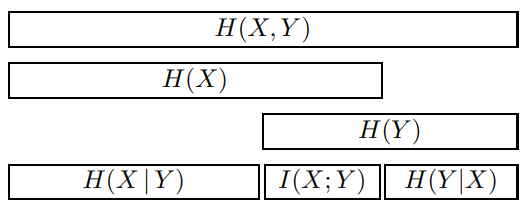
\includegraphics[width=0.7\textwidth]{images/mutua_info.png}
	\caption{Interpretazione grafica di entropia congiunta, condizionata e mutua informazione.}
\end{figure}

\textbf{Dimostrazione}:
$$
I(X;Y)=\sum_{x,y}P(x,y)\log\frac{P(x,y)}{P(x)P(y)}
=\sum_{x,y}P(x,y)\log\frac{P(x|y)P(y)}{P(x)P(y)} =
$$
$$
=\sum_{x,y}P(x,y)(\log P(x|y) + \log\frac{1}{P(x)}) 
=\sum_{x,y}P(x,y)\log\frac{1}{P(x)}+\sum_{x,y}P(x,y)\log P(x|y)
$$

la prima parte per il teorema delle probabilità totali è semplicemente:
$$
= H(x)+\sum_{x,y}P(x,y)\log P(x|y)= H(X)-\sum_{x,y}P(x,y)\log\frac{1}{P(x|y)} = H(X)-H(X|Y)
$$

\subsection{Proprietà della Mutua Informazione}
La Mutua Informazione comprende diverse proprietà:
\begin{enumerate}
	\item $I(X;X)=H(X)$ -- Dimostrazione: $H(X)-H(X|X)=H(X)$
	\item  $I(X;Y)=I(Y;X)$
	\item $I(X;Y)\ge 0$ -- Dimostrazione:\\ $$\sum_{x\in A_X}\sum_{y\in A_Y}P(x,y)\log_2\frac{P(x,y)}{P(x)P(y)}$$ poniamo: 
	$$
	\widehat{P}(x,y) = P(x,y) \quad \text{e} \quad \widehat{Q}(x,y) = P(x)P(y)
	$$
	
	e applichiamo la Diseguaglianza di Gibbs.
\end{enumerate}


\newpage

\subsubsection{Esempio N.4 - Mutua Informazione}
Supponiamo di avere le seguenti variabili aleatorie $X$ e $Y$ definite in $A=\{1, 2\}$ e con le seguenti probabilità note:\\
\begin{minipage}{0.50\textwidth}
	\begin{center}
		$$
		Pr[x=1 \wedge y=1] = 0
		$$
		$$
		Pr[x=2 \wedge y=1] = \frac{3}{4}
		$$
	\end{center}
\end{minipage}
\begin{minipage}{0.50\textwidth}
	\begin{center}
		$$
		Pr[x=1 \wedge y=2] = \frac{1}{8}
		$$
		$$
		Pr[x=2 \wedge y=2] = \frac{1}{8}
		$$
	\end{center}
\end{minipage}

Calcolare la Mutua Informazione $I(X;Y)$

Per calcolare $I(X;Y)$ devo prima calcolare $H(X)$ e $H(X|Y)$.\\ Per $H(X)$ devo calcolare $Pr(x)$ che, per il Teorema della Probabilità Totale, diventa:
$$
Pr(x) = \sum_{y} Pr[x \wedge y] = Pr[x \wedge y=1] + Pr[x \wedge y=2]
$$
Lo divido nei casi $x=1$ e $x=2$:
\begin{enumerate}
	\item $Pr[x=1] = Pr[x=1 \wedge y=1] + Pr[x=1 \wedge y=2] = 0 + \frac{1}{8} = \frac{1}{8}$
	\item $Pr[x=2] = Pr[x=2 \wedge y=1] + Pr[x=2 \wedge y=2] = 
	\frac{3}{4} + \frac{1}{8} = \frac{7}{8}$
\end{enumerate}

Adesso posso trovare $H(X)$:
$$
H(X) = \frac{1}{8}\ \log_{2}8 + \frac{7}{8}\ \log_{2} \frac{8}{7} \approx 0,375 + 0,169 = 0,544
$$
Per trovare $H(X|Y)$ calcolo prima $H(X|Y=1)$ e $H(X|Y=2)$ per poi calcolare:
$$
H(X|Y) = Pr[Y=1]\cdot H(X|Y=1) + Pr[Y=2]\cdot H(X|Y=2)
$$
So che $H(X|Y=1)$ equivale a:
$$
H(X|Y=1) = \sum_{x}\ Pr[X=x|Y=1] \log_{2} \frac{1}{Pr[X=x|Y=1]} = 
$$
$$
= Pr[x=1|y=1] \log_{2} \frac{1}{Pr[x=1|y=1]} + Pr[x=2|y=1] \log_{2} \frac{1}{Pr[x=2|y=1]} =
$$

Per il teorema della Probabilità Condizionata:\\
\begin{minipage}{0.50\textwidth}
	\begin{center}
		$$
		Pr[x=1|y=1] = \frac{Pr[x=1 \wedge y=1]}{Pr[y=1]} = 0
		$$
	\end{center}
\end{minipage}
\begin{minipage}{0.50\textwidth}
	\begin{center}
		$$
		Pr[x=2|y=1] = \frac{Pr[x=2 \wedge y=1]}{Pr[y=1]} = 1
		$$
	\end{center}
\end{minipage}
$$
H(X|Y=1) =  0 + 0 = 0
$$

Applico lo stesso ragionamento per $H(X|Y=2)$:
$$
H(X|Y=2) = Pr[x=1|y=2] \log_{2} \frac{1}{Pr[x=1|y=2]} + Pr[x=2|y=2] \log_{2} \frac{1}{Pr[x=2|y=2]}
$$

Calcolo $P[y=2]$:
$$
Pr[y=2] = Pr[y=2 \wedge x=1] + Pr[y=2 \wedge x=2] = \frac{1}{8} + \frac{1}{8} = \frac{1}{4} 
$$

Per il teorema della Probabilità Condizionata:\\
\begin{minipage}{0.50\textwidth}
	\begin{center}
		$$
		Pr[x=1|y=2] = \frac{Pr[x=1 \wedge y=2]}{Pr[y=2]} = \frac{1}{8} \cdot 4 = \frac{1}{2}
		$$
	\end{center}
\end{minipage}
\qquad
\begin{minipage}{0.50\textwidth}
	\begin{center}
		$$
		Pr[x=2|y=2] = \frac{Pr[x=2 \wedge y=2]}{Pr[y=2]} = \frac{1}{8} \cdot 4 = \frac{1}{2}
		$$
	\end{center}
\end{minipage}
$$
H(X|Y = 2) = \frac{1}{2}\cdot \log_{2} 2 + \frac{1}{2}\cdot \log_{2} 2 = 1
$$
Quindi $H(X|Y)$ equivale a:
$$
H(X|Y) = Pr[Y=1] \cdot 0 + \frac{1}{4} \cdot 1 = \frac{1}{4}
$$

Possiamo infine calcolare $I(X;Y) = H(X) - H(X|Y) = 0,544 - 0,150 = 0,394$



\chapter{Teorema del Codice Sorgente e Compressione}

\section{Massimizzare l'informazione di una variabile aleatoria}

Come abbiamo visto nella sezione precedente, l'\textbf{Informazione di Shannon} e dell'\textbf{Entropia} di una variabile aleatoria X sono essenziali per misurare l'informazione ottenuta e l'incertezza rimanente. 

Ma come possiamo \textbf{massimizzare} l'informazione ottenuta da una variabile aleatoria? E quanti bit servono per descrivere il risultato di un esperimento?

L'ideale è ottenere una strategia che massimizzi l'informazione ottenuta nel caso medio ad ogni risultato ottenuto da una v.a. e stabilire un limite inferiore di tentativi da realizzare per ottenere l'informazione intera.
Definiamo:
\begin{itemize}
	\item Il \textbf{numero} di possibili risultati con $|A_X|$
	\item Assegnamo un nome \textbf{binario} ad ogni risultato
	\item Il \textbf{raw-bit content} di $X$, ovvero la \textbf{dimensione} di ogni nome, è: $$H_0 =\log_{2}|A_X|$$
	\item Il raw-bit content corrisponde ad un \textbf{limite inferiore} per individuare il risultato di $X$.
\end{itemize}
%
Spieghiamo meglio il concetto con degli esempi pratici.

\paragraph{Gioco del 63 (o del 64)}
Il gioco consiste nell'individuare un intero $x$ compreso tra 0 e 63 (o 1 e 64) nel numero \textbf{minore} di "SI" e "NO" possibile. Come possiamo fare?

Prima di individuare la strategia ottima, associamo alle risposte "SI" e "NO" i nomi binari $\{1, 0\}$ e calcoliamo l'\textbf{entropia} (raw-bit content). Sapendo che il numero di risultati è \textbf{equiprobabile} (distribuzione uniforme), l'entropia calcolata sarà \textbf{massima}:
$$
H(X) = \log_{2} |A_X| = \log_{2} 64 = 6 
$$

Suppniamo che l'intero $x$ da indovinare sia 35, una strategia ottima è quella di usare il modulo e le potenze del due:
\begin{enumerate}
	\item È l'intero $x \geq 32$? SI $\Rightarrow 1$
	\item È l'intero $x \mod{32} \geq 16$? NO $\Rightarrow 0$
	\item È l'intero $x \mod{16} \geq 8$? NO $\Rightarrow 0$
	\item È l'intero $x \mod{8} \geq 4$? NO $\Rightarrow 0$
	\item È l'intero $x \mod{4} \geq 2$? SI $\Rightarrow 1$
	\item È l'intero $x \mod{2} = 1$? SI $\Rightarrow 1$
\end{enumerate}

Formiamo il numero: \verb|100011| $\Rightarrow 35$

Questa strategia è coerente con l'Informazione di Shannon, in quanto ad ogni tentativo svolto otteniamo:
$$
h(x) = \log_{2} \frac{1}{\frac{1}{2}} = \log_{2} 2 = 1\ \text{bit}
$$
Ed essendo 6 i tentativi, al sesto tentativo abbiamo ottenuto 6 bit, ovvero l'entropia.

Abbiamo quindi visto che l'Informazione di Shannon ha senso se i risultati della variabile aleatoria hanno la stessa probabilità. Ma continua ad avere senso se le probabilità ad ogni risultato ottenuto \textbf{cambiano}? Vediamo un altro esempio.

\paragraph{Gioco del Sottomarino}
Nella battaglia navale, ogni giocatore nasconde una flotta di navi in un mare, rappresentato con una matrice $8\times8$. Ad ogni turno, un giocatore prova a colpire le navi dell'altro giocatore colpendo uno slot della matrice. Ci sono tre possibili risultati, \verb|'mancato'|, \verb|'colpito'|, \verb|'colpito e affondato'|.

Per rappresentare l'esempio, semplifichiamo il gioco, dove ogni giocatore ha una sola nave (un sottomarino) di grandezza di un singolo slot. Ci sono quindi solo due possibili risultati:
\begin{center}
	\verb|'colpito'|, che indichiamo con \verb|'Y'|\quad e \quad \verb|'mancato'|, che indichiamo con \verb|'N'|
\end{center}

Essendo $|A_X| = 64$, l'entropia è di 6 bit, come nel gioco precedente.

Tuttavia, rispetto al gioco del 63, nel gioco del Sottomarino non abbiamo una distribuzione di probabilità uniforme, infatti:

\begin{minipage}{0.33\textwidth}
	\begin{center}
		Le probabilità al \textbf{1° lancio} sono:
		$$
		P(Y) = \frac{1}{64} \quad;\quad P(N) = \frac{63}{64}
		$$
	\end{center}
\end{minipage}
\begin{minipage}{0.33\textwidth}
	\begin{center}
		Le probabilità al \textbf{2° lancio} sono:
		$$
		P(Y) = \frac{1}{63} \quad;\quad P(N) = \frac{62}{63}
		$$
	\end{center}
\end{minipage}
\begin{minipage}{0.33\textwidth}
	\begin{center}
		Le probabilità al \textbf{3° lancio} sono:
		$$
		P(Y) = \frac{1}{62} \quad;\quad P(N) = \frac{61}{62}
		$$
	\end{center}
\end{minipage}

E così via.\\ L'informazione di Shannon ottenuta al primo tentativo, se dovessimo essere fortunati e beccare il sottomarino, sarebbe di 6 bit, ma se invece dovessimo mancarlo sarebbe:
$$
h(x) = h_1(N) = \log_{2} \frac{64}{63} = 0,0227\ \text{bit}
$$
Se mancassimo anche il secondo tentativo, l'Informazione di Shannon ottenuta sarebbe:
$$
h_2(N) = \log_{2} \frac{63}{62} = 0,0230\ \text{bit} 
$$
Se mancassimo i primi 32 tentativi, il totale di Informazione di Shannon sarebbe:
$$
\log_{2}\frac{64}{63} + \log_{2} \frac{63}{62} + \cdots + \log_{2}\frac{33}{32} = 0,0227 + 0,0230 + \cdots + 0,0430 = 1\ \text{bit}  
$$

Perché 1 bit? Perché adesso sappiamo che il sottomarino non si trova in nessuno dei 32 slot provati, che corrispondono al primo tentativo del gioco del 63. Allo stesso modo, dopo 48 tentativi falliti avremo ottenuto in tutto 2 bit di informazione. Se al 49esimo tentativo dovessimo indovinare, otterremo:
$$
h_49(Y) = \log_{2} \frac{1}{\frac{1}{16}} = \log_{2} 16 = 4\ \text{bit}
$$ 
che sommati ai 2 bit trovati prima, equivalgono ai 6 bit dell'entropia.

Supponiamo il caso peggiore, ovvero che troviamo il sottomarino al 64esimo tentativo.\\ Otterremmo ogni bit così:
\begin{enumerate}
	\item Dopo i primi 32 tentativi otterremo il 1° bit.
	\item Dopo 48 tentativi otterremo il 2° bit.
	\item Dopo 56 tentativi otterremo il 3° bit.
	\item Dopo 60 tentativi otterremo il 4° bit.
	\item Dopo 62 tentativi otterremo il 5° bit.
	\item Dopo 63 tentativi otterremo il 6° bit. Rimarrà un singolo slot libero, che sarà la posizione del sottomarino.
\end{enumerate}

Possiamo affermare che l'Informazione di Shannon, indipendentemente dalla distribuzione di probabilità, continua ad avere senso per misurare l'informazione ricavata da un evento.

\newpage
\section{Introduzione alla compressione}
Adesso possiamo discutere di quanti bit sono \textbf{necessari} per descrivere il risultato di un evento sorgente.
Dimostrare che è possibile comprimere i dati da una particolare sorgente in un file a $L$ bit per simbolo e ricostruire i dati in maniera affidabile equivale a dimostrare che il contenuto di informazione media di quella sorgente è al più $L$ bit per simbolo.

Utilizzeremo le nozioni base del Teorema del Codice Sorgente per la \textbf{compressione di una sorgente}. Esistono \textbf{due modi} per comprimere una sorgente:
\begin{enumerate}
	\item \textbf{Compressione Lossy}: Questo tipo di compressione consente la \textbf{perdita di informazione} per comprimere il file sorgente. Un compressore lossy comprime quindi alcuni file ma ne \textbf{mappa altri alla stessa codifica}.\\ Denoteremo con $\delta$ la probabilità di fallimento del compressore lossy. Se $\delta$ può essere ridotto ad un valore molto basso, il compressore può rivelarsi utile.
	
	\item \textbf{Compressione Lossless}: Questo tipo di compressione \textbf{non consente alcun tipo di perdita di informazione}. Un compressore lossless mappa tutti i file a \textbf{codifiche diverse}, con la conseguenza che alcuni file potrebbero \textbf{ingrandirsi} invece che ridursi.\\
	Vogliamo quindi creare un compressore dove la probabilità che un file si ingradisca sia \textbf{molto bassa} e quella in cui si riduca sia \textbf{molto elevata}.
\end{enumerate}

\section{Compressione Lossy}
Come possiamo creare una strategia di compressione lossy?
Indipendentemente dal tipo di compressore che vogliamo costruire, abbiamo bisogno di conoscere le probabilità di ogni possibile risultato.

Supponiamo di voler comprimere un \textbf{file di testo} formato da caratteri ASCII di un alfabeto $A_X$.\\ In un generico testo in inglese o in italiano con molta probabilità ci sono caratteri \textbf{molto utilizzati} e altri invece \textbf{molto meno}, che quindi possono essere rimossi dall'alfabeto $A_X$ per creare un alfabeto ridotto $A_X'$.

Potremmo quindi calcolare il \textbf{raw-bit content} degli alfabeti $A_X$ e $A_X'$ per vedere quanto \textbf{spazio risparmiamo}. Più caratteri siamo disposti a rimuovere, più la probabilità $\delta$ aumenta.

\textbf{Esempio N.1 - Compressione Lossy di un Alfabeto $A_X$}

Supponiamo di avere un alfabeto $A_X$ formato da questi caratteri e le rispettive probabilità:
$$
A_X = \{\verb|a, b, c, d, e, f, g, h|\}\qquad\qquad P_X = \left\{\frac{1}{4}, \frac{1}{4}, \frac{1}{4}, \frac{3}{16}, \frac{1}{64}, \frac{1}{64}, \frac{1}{64}, \frac{1}{64}\right\}
$$

Calcoliamo il \textbf{raw-bit content} di $A_X$:
$$
H_0(X) = \log_{2} 8 = 3\ \text{bit}
$$

Vogliamo comprimere l'alfabeto $A_X$ eliminando i caratteri poco probabili, ovvero $\{\verb|e,f,g,h|\}$.

Abbiamo così un alfabeto $A_X'$ formato da $\{\verb|a,b,c,d|\}$, il cui raw-bit content è $H_0(X') = \log_2 4 = 2\ \text{bit}$ e un $\delta = \frac{1}{16}$.

Per formalizzare una strategia di compressione con un rischio $\delta$, creiamo il più piccolo insieme $S_\delta$ affinché la probabilità che $x$ non sia in $S_\delta$ è:

\begin{equation}
	Pr(x\notin S_\delta) \leq \delta
\end{equation}

\newpage
\subsection{Strumenti per la compressione lossy}
Definiamo due \textbf{strumenti fondamentali} per una compressione lossy ideale:
\begin{itemize}
	\item \textbf{Minimo insieme $\delta$-sufficiente}: Minimo sottoinsieme $S_\delta \subseteq A_X$ tale che:
	\begin{equation}
		Pr(x \in S_\delta) \geq 1 - \delta
	\end{equation}
	Questo sottoinsieme $S_\delta$ viene costruito in maniera greedy, ordinando gli elementi di $A_X$ in ordine decrescente in base alla loro probabilità ed aggiungendoli ad $S_\delta$ partendo da quelli più probabili, fino a quando la probabilità totale è $\geq 1 - \delta$. Possiamo infine assegnare un nome binario ad ogni elemento di $S_\delta$.
	
	\item \textbf{Essential bit content} di $X$ equivale a:
	\begin{equation}
		H_\delta(X) = \log_{2} |S_\delta|
	\end{equation}
	ed è la lunghezza delle codifiche di $S_\delta$.\\
	\textit{Osservazione}: Se $\delta=0$ l'essential bit content \textbf{coincide} con il raw-bit content.
\end{itemize}


\textbf{Esempio N.2 - Compressione lossy di blocchi di bit}

Supponiamo una variabile aleatoria $X$ che può assumere i valori
$x_i \in \{0,1\}$ con:
\begin{itemize}
	\item $Pr[x_i = 0] = p_0 = 0.9$
	\item $Pr[x_i = 1] = p_1 = 0.1$
\end{itemize}

Suppondendo una stringa di 4 bit, a quanto equivale l'\textbf{essential bit content} di questa stringa?

Prendiamo in considerazione \textbf{i casi possibili}:
\begin{enumerate}
	\item $Pr[X=0000]= p_0^4 = 0,6561$
	\item $P[X=\text{"x contiene un 1"}] = 4 \cdot (p_0^3\cdot p_1) = 4 \cdot 0,0729 = 0,3036$
	\item $P[X=\text{"x contiene due 1"}]= 6 \cdot (p_0^2 \cdot p_1^2) = 6\cdot 0,0081 = 0,0486$
	\item $P[X=\text{"x contiene tre 1"}]= 4 \cdot (p_0 \cdot p_1^3) = 4 \cdot 0,0009 = 0,0036$
	\item $P[X=1111]=0,00014$
\end{enumerate}

Essendo $A_X = 16$, calcolo il raw-bit content: $H_0(X) = \log_{2} 16 = 4\ \text{bit}$

Di conseguenza, per una compressione lossy efficace, potremmo sicuramente eliminare i casi 4 e 5 e mantenere i casi 1 e 2.
Abbiamo due opzioni con il caso 3:
\begin{itemize}
	\item Se lo mantenessimo, avremmo: 
	$$Pr[X= \text{"x contiene al massimo due 1"}] > 0,99$$ 
	e un $\delta = 0,01$. Sapendo quindi che $|S_\delta| = 11$ posso calcolare l'essential bit content:
	$$
	H_\delta(X^{11}) = \log_{2} 11 = 3,45\ \text{bit}
	$$
	Mantenendo il caso 3 ho risparmiato solamente 0,55 bit.
	
	\item Se lo rimuovessimo, avremmo:
	$$Pr[X= \text{"x contiene al massimo un 1"}] > 0,94$$ 
	e un $\delta = 0,06$. Sapendo quindi che $|S_\delta| = 5$ posso calcolare l'essential bit content:
	$$
	H_\delta(X^5) = \log_{2} 5 = 2,32\ \text{bit}
	$$
	Rimuovendo il caso 3 ho risparmiato 1,68 bit, un risparmio più consistente, con un $\delta$ sempre basso.
\end{itemize}

\newpage
Da questo esempio possiamo constatare che $H_\delta(X^N)$ \textbf{dipenda troppo} dal parametro $\delta$, un comportamento che dovremmo evitare. Questo tuttavia succede solo con un $N$ \textbf{piccolo} infatti, al crescere di $N$, $H_\delta(X^N)$ diventa sempre meno dipendente da $\delta$.

Possiamo quindi normalizzare rispetto alla lunghezza $N$ di una qualsiasi stringa binaria: $\frac{1}{N}H_\delta(x^N)$
\begin{minipage}{0.50\textwidth}
	\begin{figure}[H]
		\centering
		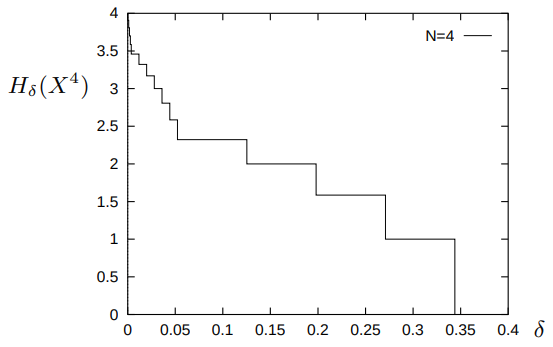
\includegraphics[width=0.9\textwidth]{images/lossy1.png}
	\end{figure}
\end{minipage}
\begin{minipage}{0.50\textwidth}
	\begin{figure}[H]
		\centering
		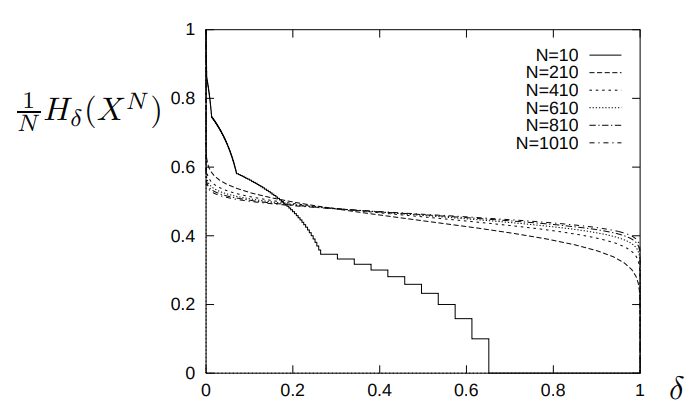
\includegraphics[width=1\textwidth]{images/lossy2.png}
	\end{figure}
\end{minipage}

Questo fenomeno è detto \textbf{Tipicalità}, cioè al crescere di $N$ la stringa più probabile aumenta il proprio peso e ci si avvicina al comportamento tipico.


\subsection{Teorema del Codice Sorgente di Shannon}
Data una variabile aleatoria $X$ con un'entropia $H(X) = H\ \text{bit}$, un $\varepsilon > 0$ e $0 < \delta < 1$ allora esiste $N_0 \in \mathbb{N}^+$ tale che, per $N > N_0$ vale:
\begin{equation}
	\left| \frac{1}{N} H_\delta(X^N)-H \right| < \varepsilon	
\end{equation}
Di conseguenza:
$$
H - \varepsilon < \frac{1}{N} H_\delta(X^N) < H + \varepsilon
$$

Da questo teorema possiamo dedurre due importanti risultati:
\begin{enumerate}
	\item Il primo deriva da: $$\frac{1}{N} H_\delta(X^N) < H + \varepsilon$$
	che afferma che anche per $\delta$ molto piccoli, il numero di bit per simbolo $\frac{1}{N} H_\delta(X^N)$ necessario per specificare una stringa $x$ con $N$ simboli con probabilità di errore bassa non deve eccedere gli $H + \varepsilon$ bit. Abbiamo bisogno di una \textbf{piccola tolleranza} per errore e il numero di bit richiesti crolla da $H_0(X)$ a $(H+\varepsilon)$. 
	
	\item Il secondo deriva da: $$H - \varepsilon < \frac{1}{N} H_\delta(X^N)$$
	che afferma che anche se il nostro compressore fosse molto tollerante agli errori di compressione, con un $\delta$ vicino a 1, il \textbf{numero medio} di bit per simbolo necessari per rappresentare $x$ devono essere almeno $H - \varepsilon$ bit.
\end{enumerate}

Questi due estremi quindi affermano che, indipendentemente dalla nostra tolleranza all'errore, il numero di bit per simbolo necessari per rappresentare $x$ è $H$ bit.

\newpage
\section{Compressione lossless}

A differenza della compressione lossy, dove i blocchi di codice avevano \textbf{lunghezza fissa} e venivano compressi con la \textbf{stessa codifica}, nella compressione lossless ogni file ha \textbf{lunghezza variabile} e per ogni file vengono usate \textbf{codifiche diverse} con la garanzia di comprimere e decomprimere \textbf{senza errori}.

L'idea è quella di poter comprimere, in media, assegnando codifiche \textbf{più brevi} a simboli/risultati \textbf{più probabili} e codifiche \textbf{più lunghe} a simboli/risultati \textbf{meno probabili}. Questo approccio non è tuttavia esente da difetti:
\begin{enumerate}
	\item Se alcuni codici simbolici sono accorciati, di quanto gli altri codici potrebbero essere allungati?
	\item Come possiamo assicurarci che un codice simbolico sia facile da decodificare?
	\item Come possiamo arrivare alla miglior compressione di un codice?
\end{enumerate}

\textbf{Notazione per gli alfabeti}
\begin{itemize}
	\item $A^N$ denota l'insieme delle N-tuple ordinate di elementi di $A$. Esempio:
	$$
	\{0,1\}^3 = \{000,001,010,011,100,101,110,111\}
	$$
	\item $A^*$ denota l'insieme delle stringhe di lunghezza finita su $A$. Esempio:
	$$
	\{0,1\}^* = \{0,1,00,01,10,11,000,001,\cdots\}
	$$
\end{itemize}

\subsection{Codici Simbolici}
\subsubsection{Definizioni di Codice Simbolico e Codice Esteso}
Un \textbf{codice simbolico} (binario) $C$ di una variabile aleatoria $X$ è una mappatura dei valori\\ $A_X = \{a_1, \cdots, a_n\} \rightarrow \{0,1\}^*$. Denotiamo con $c(x)$ ogni \textit{codeword} che corrisponde ad $x$ e con $l(x)$ denotiamo la \textbf{lunghezza} della codifica.

Il \textbf{codice esteso} può essere visto come una mappa da $A_X^* \rightarrow \{0,1\}^*$ ottenuto per \textbf{concatenazione} delle codeword corrispondenti (senza punteggiatura):
\begin{equation}
	c^*:A_X^*\rightarrow \{0,1\}^* \quad , \quad c^*(x_1 x_2 \cdots x_N) = c(x_1)c(x_2)\cdots c(x_N)
\end{equation}

Affinché un codice simbolico sia utile deve rispecchiare tre requisiti:
\begin{enumerate}
	\item Dev'essere \textbf{Univocamente Decodificabile}.
	\item Dev'essere facile da decodificare.
	\item Dev'essere compresso il più possibile.
\end{enumerate}

\subsubsection{Definizione di Codice Univocamente Decodificabile}
Un codice simbolico $x(X)$ è \textbf{univocamente decodificabile} se il corrispondente codice esteso $C^*(X)$ è tale che non esistano due stringhe distinte con la stessa codifica:
$$
\forall x,y \in A_X^*\ ,\ x \neq y \Rightarrow c^*(x) \neq c^*(y)
$$

\textbf{Esempio N.1 - Codice univocamente decodificabile}

Dato un codice simbolico per una variabile aleatoria $X$ definito in:\\
\begin{minipage}{0.50\textwidth}
	$$
	A_X = \{\verb|a, b, c, d|\}\qquad P_X = \left\{\frac{1}{2}, \frac{1}{4}, \frac{1}{8}, \frac{1}{8}
	\right\}
	$$
\end{minipage}
\begin{minipage}{0.50\textwidth}
	\begin{table}[H]
		\centering
		\begin{tabular}{c|cc}
			$a_i$ & $c(a_i)$ & $l_i$ \\
			\hline
			$a$ & 1000 & 4 \\
			$b$ & 0100 & 4 \\
			$c$ & 0010 & 4 \\
			$d$ & 0001 & 4 \\
		\end{tabular}
	\end{table}
\end{minipage}

Usando il codice esteso, potremmo codificare la stringa \verb|acdbac| come:
$$
c^*(\verb|acdbac|) = \verb|100000100001010010000010|.
$$
Questa codifica è \textbf{univocamente decodificabile}.

\newpage

\textit{OSSERVAZIONE}: Un codice simbolico è più semplice da decodificare se è possibile identificarne la fine di una codeword non appena essa si presenta, ciò significherebbe che \textbf{nessuna codeword può essere prefisso di un'altra}.

\subsection{Codici Prefix-free}
Una stringa $c$ è \textbf{prefisso} di un'altra $d$ se esiste una stringa-coda (o suffisso) $s$ tale che: $cs = d$.\\
Esempio: 1 e 10 sono entrambi prefisso di 101.

\subsubsection{Definizione di Codice Prefix-free}
Un codice simbolico è detto \textbf{Prefix-free} se nessuna codeword è prefisso di un'altra.
\begin{itemize}
	\item I codici prefix-free sono anche chiamati \textbf{istantanei} o \textbf{autopunteggiati}.
	\item I codici prefix-free sono \textbf{univocamente decodificabili}.
	\item I codici prefix-free sono associati a degli \textbf{alberi binari}, che possono essere incompleti se l'albero ha rami non utilizzati e completi se invece ogni ramo è usato.
\end{itemize}

\textbf{Esempio N.2 - Codici Prefix-free}

\begin{enumerate}
	\item Il codice $C_1 = \{0, 101\}$ è prefix-free e l'albero che forma è incompleto.
	\begin{center}
		\begin{tikzpicture}[scale=0.12]
			\tikzstyle{every node}+=[inner sep=0pt]
			\draw [black] (37.4,-14.3) circle (3);
			\draw (37.4,-14.3) node {$R$};
			\draw [black] (30.9,-24) circle (3);
			\draw (30.9,-24) node {$0$};
			\draw [black] (44.1,-24) circle (3);
			\draw (44.1,-24) node {$-$};
			\draw [black] (49.7,-33.1) circle (3);
			\draw (49.7,-33.1) node {$-$};
			\draw [black] (38.1,-33.1) circle (3);
			\draw (38.1,-33.1) node {$-$};
			\draw [black] (31.6,-42.5) circle (3);
			\draw (31.6,-42.5) node {$-$};
			\draw [black] (44.1,-42.5) circle (3);
			\draw (44.1,-42.5) node {$101$};
			\draw [black] (35.73,-16.79) -- (32.57,-21.51);
			\fill [black] (32.57,-21.51) -- (33.43,-21.12) -- (32.6,-20.56);
			\draw (33.54,-17.81) node [left] {$0$};
			\draw [black] (39.1,-16.77) -- (42.4,-21.53);
			\fill [black] (42.4,-21.53) -- (42.35,-20.59) -- (41.53,-21.16);
			\draw (41.35,-17.79) node [right] {$1$};
			\draw [black] (45.67,-26.55) -- (48.13,-30.55);
			\fill [black] (48.13,-30.55) -- (48.13,-29.6) -- (47.28,-30.13);
			\draw (47.53,-27.27) node [right] {$1$};
			\draw [black] (42.45,-26.5) -- (39.75,-30.6);
			\fill [black] (39.75,-30.6) -- (40.61,-30.2) -- (39.77,-29.65);
			\draw (40.49,-27.22) node [left] {$0$};
			\draw [black] (36.39,-35.57) -- (33.31,-40.03);
			\fill [black] (33.31,-40.03) -- (34.17,-39.66) -- (33.35,-39.09);
			\draw (34.25,-36.44) node [left] {$0$};
			\draw [black] (39.71,-35.63) -- (42.49,-39.97);
			\fill [black] (42.49,-39.97) -- (42.48,-39.03) -- (41.63,-39.57);
			\draw (41.72,-36.49) node [right] {$1$};
		\end{tikzpicture}
	\end{center}
	
	\item Il codice $C_2 = \{1, 101\}$ \textbf{non è} prefix-free, tuttavia è univocamente decodificabile.
	
	\item Il codice $C_3 = \{0, 10, 110, 111\}$ è prefix-free e l'albero che forma è completo.
	\begin{center}
		\begin{tikzpicture}[scale=0.12]
			\tikzstyle{every node}+=[inner sep=0pt]
			\draw [black] (37.4,-14.3) circle (3);
			\draw (37.4,-14.3) node {$R$};
			\draw [black] (30.9,-24) circle (3);
			\draw (30.9,-24) node {$0$};
			\draw [black] (44.1,-24) circle (3);
			\draw (44.1,-24) node {$-$};
			\draw [black] (49.7,-33.1) circle (3);
			\draw (49.7,-33.1) node {$-$};
			\draw [black] (38.1,-33.1) circle (3);
			\draw (38.1,-33.1) node {$10$};
			\draw [black] (56.3,-41.9) circle (3);
			\draw (56.3,-41.9) node {$111$};
			\draw [black] (43.3,-41.9) circle (3);
			\draw (43.3,-41.9) node {$110$};
			\draw [black] (35.73,-16.79) -- (32.57,-21.51);
			\fill [black] (32.57,-21.51) -- (33.43,-21.12) -- (32.6,-20.56);
			\draw (33.54,-17.81) node [left] {$0$};
			\draw [black] (39.1,-16.77) -- (42.4,-21.53);
			\fill [black] (42.4,-21.53) -- (42.35,-20.59) -- (41.53,-21.16);
			\draw (41.35,-17.79) node [right] {$1$};
			\draw [black] (45.67,-26.55) -- (48.13,-30.55);
			\fill [black] (48.13,-30.55) -- (48.13,-29.6) -- (47.28,-30.13);
			\draw (47.53,-27.27) node [right] {$1$};
			\draw [black] (42.45,-26.5) -- (39.75,-30.6);
			\fill [black] (39.75,-30.6) -- (40.61,-30.2) -- (39.77,-29.65);
			\draw (40.49,-27.22) node [left] {$0$};
			\draw [black] (51.5,-35.5) -- (54.5,-39.5);
			\fill [black] (54.5,-39.5) -- (54.42,-38.56) -- (53.62,-39.16);
			\draw (53.58,-36.1) node [right] {$1$};
			\draw [black] (47.94,-35.53) -- (45.06,-39.47);
			\fill [black] (45.06,-39.47) -- (45.94,-39.12) -- (45.13,-38.53);
			\draw (45.91,-36.12) node [left] {$0$};
		\end{tikzpicture}
	\end{center}
	
	\item Il codice $C_4 = \{00, 01, 10, 11\}$ è prefix-free e l'albero che forma è completo.
	\begin{center}
		\begin{tikzpicture}[scale=0.12]
			\tikzstyle{every node}+=[inner sep=0pt]
			\draw [black] (37.4,-14.3) circle (3);
			\draw (37.4,-14.3) node {$R$};
			\draw [black] (27.6,-24) circle (3);
			\draw (27.6,-24) node {$-$};
			\draw [black] (47.7,-24) circle (3);
			\draw (47.7,-24) node {$-$};
			\draw [black] (55,-33.8) circle (3);
			\draw (55,-33.8) node {$11$};
			\draw [black] (42.8,-33.8) circle (3);
			\draw (42.8,-33.8) node {$10$};
			\draw [black] (33.9,-33.8) circle (3);
			\draw (33.9,-33.8) node {$01$};
			\draw [black] (21.7,-33.8) circle (3);
			\draw (21.7,-33.8) node {$00$};
			\draw [black] (35.27,-16.41) -- (29.73,-21.89);
			\fill [black] (29.73,-21.89) -- (30.65,-21.68) -- (29.95,-20.97);
			\draw (31.48,-18.67) node [above] {$0$};
			\draw [black] (39.58,-16.36) -- (45.52,-21.94);
			\fill [black] (45.52,-21.94) -- (45.28,-21.03) -- (44.59,-21.76);
			\draw (43.57,-18.67) node [above] {$1$};
			\draw [black] (49.49,-26.41) -- (53.21,-31.39);
			\fill [black] (53.21,-31.39) -- (53.13,-30.45) -- (52.33,-31.05);
			\draw (51.93,-27.51) node [right] {$1$};
			\draw [black] (46.36,-26.68) -- (44.14,-31.12);
			\fill [black] (44.14,-31.12) -- (44.95,-30.62) -- (44.05,-30.18);
			\draw (44.55,-27.79) node [left] {$0$};
			\draw [black] (29.22,-26.52) -- (32.28,-31.28);
			\fill [black] (32.28,-31.28) -- (32.27,-30.33) -- (31.42,-30.87);
			\draw (31.37,-27.59) node [right] {$1$};
			\draw [black] (26.05,-26.57) -- (23.25,-31.23);
			\fill [black] (23.25,-31.23) -- (24.09,-30.8) -- (23.23,-30.29);
			\draw (24.01,-27.63) node [left] {$0$};
		\end{tikzpicture}
	\end{center}
\end{enumerate}

\subsubsection{Definizione di Lunghezza Attesa}
La lunghezza attesa $L(C, X)$ di un codice simbolico $C$ per una variabile aleatoria $X$ è:
\begin{equation}
	L(C,X) = \sum_{x\in A_X} P(x)\cdot l(x) = \sum_{i=1}^{I} p_i\cdot l_i \qquad \text{dove}\ I = |A_X|
\end{equation}

\textbf{Esempio N.3 - Entropia e Lunghezza Attesa di un codice prefix-free}

Dato il codice simbolico $C_3$ (del precedente esempio) per una variabile aleatoria $X$ definito in:\\
\begin{minipage}{0.50\textwidth}
	$$
	A_X = \{\verb|a, b, c, d|\}\qquad P_X = \left\{\frac{1}{2}, \frac{1}{4}, \frac{1}{8}, \frac{1}{8}
	\right\}
	$$
\end{minipage}
\begin{minipage}{0.50\textwidth}
	\begin{table}[H]
		\centering
		\renewcommand{\arraystretch}{1.5}
		\begin{tabular}{c|c|c|c|c}
			$a_i$ & $c(a_i)$ & $p_i$ & $h(p_i)$ & $l(a_i)$ \\
			\hline
			$a$ & 0 & $\frac{1}{2}$ & 1 & 1 \\
			$b$ & 10 & $\frac{1}{4}$ & 2 & 2 \\
			$c$ & 110 & $\frac{1}{8}$ & 3 & 3 \\
			$d$ & 111 & $\frac{1}{8}$ & 3 & 3 \\
		\end{tabular}
	\end{table}
\end{minipage}

Calcoliamo l'entropia e la lunghezza attesa.
$$
H(X) = \frac{1}{2} \log_2 2+ \frac{1}{4} \log_2 4+ \frac{1}{8} \log_2 8+ \frac{1}{8} \log_2 8 = \frac{1}{2} + 2 \cdot \frac{1}{4} + 3 \cdot \frac{1}{4} = 1 + \frac{3}{4} = 1.75\ \text{bit}
$$
$$
L(C_3, X) = \frac{1}{2} \cdot 1 + \frac{1}{4} \cdot 2 + \frac{1}{8} \cdot 3 + \frac{1}{8} \cdot 3 = 1 + \frac{3}{4} = 1.75\ \text{bit}
$$

Il codice $C_3$ è prefix-free e $L(C_3, X) = H(X)$

\textbf{Esempio N.4 - Entropia e Lunghezza attesa di un codice non univocamente decodificabile}

Dato il codice simbolico $C_5 = \{0, 1, 10, 11\}$ per una variabile aleatoria $X$ definito in:\\
\begin{minipage}{0.50\textwidth}
	$$
	A_X = \{\verb|a, b, c, d|\}\qquad P_X = \left\{\frac{1}{2}, \frac{1}{4}, \frac{1}{8}, \frac{1}{8}
	\right\}
	$$
\end{minipage}
\begin{minipage}{0.50\textwidth}
	\begin{table}[H]
		\centering
		\renewcommand{\arraystretch}{1.5}
		\begin{tabular}{c|c|c|c|c}
			$a_i$ & $c(a_i)$ & $p_i$ & $h(p_i)$ & $l(a_i)$ \\
			\hline
			$a$ & 0 & $\frac{1}{2}$ & 1 & 1 \\
			$b$ & 1 & $\frac{1}{4}$ & 2 & 1 \\
			$c$ & 10 & $\frac{1}{8}$ & 3 & 2 \\
			$d$ & 11 & $\frac{1}{8}$ & 3 & 2 \\
		\end{tabular}
	\end{table}
\end{minipage}

Calcoliamo l'entropia e la lunghezza attesa.
$$
H(X) = 1.75\ \text{bit} \quad  L(C_5, X) = \frac{1}{2} \cdot 1 + \frac{1}{4} \cdot 2 + \frac{1}{8} \cdot 2 + \frac{1}{8} \cdot 2 = \frac{1}{2} + \frac{3}{4} = 1.25\ \text{bit}
$$

Il codice $C_5$ non solo non è prefix-free, ma non è nemmeno univocamente decodificabile e \\$L(C_5, X) < H(X)$

\textbf{Esempio N.5 - Entropia e Lunghezza attesa di un codice non prefix-free}

Dato il codice simbolico $C_6 = \{0, 01, 011, 111\}$ per una variabile aleatoria $X$ definito in:\\
\begin{minipage}{0.50\textwidth}
	$$
	A_X = \{\verb|a, b, c, d|\}\qquad P_X = \left\{\frac{1}{2}, \frac{1}{4}, \frac{1}{8}, \frac{1}{8}
	\right\}
	$$
\end{minipage}
\begin{minipage}{0.50\textwidth}
	\begin{table}[H]
		\centering
		\renewcommand{\arraystretch}{1.55}
		\begin{tabular}{c|c|c|c|c}
			$a_i$ & $c(a_i)$ & $p_i$ & $h(p_i)$ & $l(a_i)$ \\
			\hline
			$a$ & 0 & $\frac{1}{2}$ & 1 & 1 \\
			$b$ & 01 & $\frac{1}{4}$ & 2 & 2 \\
			$c$ & 011 & $\frac{1}{8}$ & 3 & 3 \\
			$d$ & 111 & $\frac{1}{8}$ & 3 & 3 \\
		\end{tabular}
	\end{table}
\end{minipage}

Calcoliamo l'entropia e la lunghezza attesa.
$$
H(X) = 1.75\ \text{bit} \quad  L(C_6, X) = \frac{1}{2} \cdot 1 + \frac{1}{4} \cdot 2 + \frac{1}{8} \cdot 3 + \frac{1}{8} \cdot 3 = 1 + \frac{3}{4} = 1.75\ \text{bit}
$$

Il codice $C_6$ non è prefix-free ma univocamente decodificabile e $L(C_6, X) = H(X)$.

Ma quali sono i limiti imposti dall'univoca decodificabilità?\\ Data una lista di interi $\{l_i\}$, esiste un codice univocamente decodificabile con lunghezze $l_i$?

Possiamo rispondere a queste domande grazie alla \textbf{Disuguaglianza di Kraft}

\newpage

\subsection{Disuguaglianza di Kraft}
\subsubsection{Definizione di Disuguaglianza di Kraft}
Per ogni codice univocamente decodificabile $C(X)$ sull'alfabeto binario $\{0,1\}$, le lunghezze delle codeword devono soddisfare:
\begin{equation}
	\sum_{i=1}^{I} 2^{-l_i} \leq 1 \qquad \text{dove}\ I = |A_X| 
\end{equation}

Se un codice univocamente decodificabile soddisfa la Disuguaglianza di Kraft con \textbf{uguaglianza}, allora si dice che quel codice è \textbf{completo}.

\textbf{Dimostrazione}

Definiamo $\sum_{i=1}^{I} 2^{l_i}$ e sia:
$$
S^N = \left[\sum_{i=1}^{I} 2^{l_i}\right]^N = \sum_{i_1 = 1}^{I} \sum_{i_2 = 1}^{I} \cdots \sum_{i_N = 1}^{I} 2^{-(l_{i_1} + l_{i_2} + \cdots l_{i_N})}
$$

La quantità dell'esponente, $(l_{i_1} + l_{i_2} + \cdots l_{i_N})$ è la lunghezza della codifica di una stringa $x = a_{i_1}\ a_{i_2}\cdots a_{i_N}$ e, per ognuna di tali stringhe, c'è un termine di questa somma.\\
Introduciamo un array $A_l$ che conta quante stringhe $x$ hanno lunghezza $l$.\\ Successivamente definiamo $l_{min} = min_i\cdot l_i$ e $l_{max} = max_i \cdot l_i$ tali che:
$$
S^N = \sum_{l=N\cdot l_{min}}^{N\cdot l_{max}} 2^{-l} A_l
$$

Poiché il codice C è univocamente decodificabile le codeword sono \textbf{tutte distinte} e quindi ci sono al più $2^l$ stringhe di lunghezza $l$, con $$A_l \leq 2^l$$

Allora:
$$
S^N = \sum_{l=N\cdot l_{min}}^{N\cdot l_{max}} 2^{-l} A_l \leq \sum_{l=N\cdot l_{min}}^{N\cdot l_{max}} 1 \leq N \cdot l_{max} \quad ,\ \forall N
$$

Se $S$ fosse $>1$ allora: $$S^N \leq N \cdot l_{max}$$
il ché è un assurdo, in quando $S^N$ ha crescita esponenziale mentre $N \cdot l_{max}$ crescita polinomiale.

\subsubsection{Disuguaglianza di Kraft per codici Prefix-free}
Dato un insieme di lunghezze che soddisfano:
$$
\sum_{i=1}^{I} 2^{-l_i} \leq 1
$$
esiste un codice prefix-free con queste lunghezze delle codeword.

\textbf{Dimostrazione}

Usiamo una strategia greedy. Date le lunghezze $l_1 \leq l_2 \leq \cdots \leq l_I$ consideriamo un albero binario con profondità $l_n = l_{max}$ e $2^{l_max}$ foglie. Diremo che un nodo al livello $l$ è disponbile se non è ancora stato scelto né è un discendente di un nodo scelto.

Al passo $i$:
\begin{itemize}
	\item Consideriamo un nodo $v$ con profondità $\leq l_i$. Se ha profondità $< l_i$, espandiamolo aggiungendo i suoi figli. Ripetiamo finché non arriviamo a profondità $l_i$
	\item Assegnamo $v$ come i-esima codeword. $v$ e i suoi discendenti non sono più disponibili.
\end{itemize}

Dopo aver assegnato le prime $i-1$ parole, il peso dei nodi disponibili è:
$$
W_i = \sum_{v} 2^{-depth(v)}\quad\text{con}\ v\ \text{disponibili}  
$$

\newpage

Affermo che $W_i \geq 2^{l_i}\ \forall i$ e pertanto al passo $i$ esiste almeno un nodo utilizzabile. Dimostriamo questa affermazione per induzione.

\textbf{Caso Base}: All'inizio l'unico nodo disponibile è la radice:
$$
W_1 = 2^0 = 1 \geq 2^{l_1}\quad,\ l_1 \geq 1
$$

\textbf{Passo Induttivo}: Supponiamo che l'affermazione sia vero fino al all'($i-1$)-esimo passo.

Al passo $i$, scegliamo un nodo $v$ a profondità $l_i$, che contribuisce con $2^{-l_i}$ al peso. Quindi:
$$
W_{i+1} = W_i - 2^{-l_i}
$$

Vogliamo $$W_{i+1} \geq 2^{-l_{i+1}}$$

Dalla diseguaglianza di Kraft applicata a tutti gli $n$ termini
$$
\sum_{j=1}^{n} 2^{-l_j} \leq 1 = W_1	\quad \text{e} \quad W_i = W_1 - \sum_{j=1}^{i-1} 2^{-l_j}
$$
quindi
$$
W_{i+1} = W_1 - \sum_{j=1}^{i} 2^{-l_j} \geq \sum_{j=i+1}^{n} 2^{-l_j} \geq 2^{-l_{i+1}}
$$

\subsection{Quanto possiamo comprimere una sorgente?}
\subsubsection{Limite inferiore	della lunghezza attesa}
La lunghezza $L(C,X)$ di un codice $C$ univocamente decodificabile è: 
\begin{equation}
	L(C,X) \geq H(X)
\end{equation}

\textbf{Dimostrazione}:

Definiamo le \textit{probabilità implicite}: 
$$
q_i = \frac{2^{-l_i}}{z}\quad \text{con} \quad z=\sum_{i} 2^{-l_i}
$$
affinché: 
$$
l_i = \frac{\log_{2} 1}{q_i - \log_{2} z}
$$
Usiamo quindi la diseguaglianza di Gibbs, per cui diventa:
$$
\sum_{i} p_i \log_{2} \frac{1}{q_i} \geq \sum_{i} p_i \log_2 \frac{1}{p_i}\quad \text{e vale se}\ q_i = p_i
$$
Infine con la diseguaglianza di Kraft con $z \leq 1$:
$$
L(C,X) = \sum_{i} p_i\cdot l_i = \sum_{i} p_i (\log_{2}\frac{1}{q_i} - \log_2 z) \geq \sum_{i} p_i (\log_{2}\frac{1}{p_i} - \log_2 z) \geq H(X)
$$

\subsubsection{Codice simbolico ottimo}
Se la lunghezza attesa è minimizzata ed è uguale all'entropia solo se le lunghezze delle codeword sono uguali all'Informazione di Shannon:
$$
l_i = \log_{2}\frac{1}{p_i}\quad \text{allora}\quad L(C,X)= H(X)
$$

\newpage
\subsubsection{Teorema del Codice Sorgente per Codici Simbolici}
Data una variabile aleatoria $X$ esiste un codice prefix-free $C$ la cui lunghezza attesa soddisfa:
\begin{equation}
	H(X) \leq L(C,X) \leq H(X) + 1
\end{equation}

\textbf{Dimostrazione}:

Arrotondiamo per \textbf{eccesso} le lunghezze delle codeword rispetto alla loro lunghezza \textbf{ottimale}: $$l_i = \ceil{\log_{2}\left(\frac{1}{p_i}\right)}$$
Controlliamo che la diseguaglianza di Kraft sia soddisfatta:
$$
\sum_{i=1}^{I} 2^{-l_i} = \sum_{i=1}^{I} 2^{-\ceil{\log_{2}(\frac{1}{p_i})}} \leq \sum_{i=1}^{I} 2^{-\log_{2}\frac{1}{p_i}} \leq \sum_{i=1}^{I} p_i = 1
$$
Calcoliamo:
$$
H(X) \leq L(C,X) = \sum_{i=1}^{I} p_i l_1 = \sum_{i=1}^{I} p_i \ceil{\log_{2}\frac{1}{p_i}} < \sum_{i} p_i (\log_{2} \frac{1}{p_i} + 1) = H(X) + 1
$$

\textit{OSSERVAZIONE}: Se usiamo un codice le cui probabilità sono $\{p_i\}_{i=1}^I$ e usiamo un codice completo con lunghezze $l_i$, esse ci definiscono le probabilità di un codice ottimale $q_i = 2^{-l_i}$.\\
La loro lunghezza attesa sarà:
$$
L(C,X) = H(X) + \sum_{i} p_i \log_{2}\frac{p_i}{q_i}
$$
con $\sum_{i} p_i \log_{2}\frac{p_i}{q_i}$ = $D_{KL}(P||Q)$ (Divergenza di Kullback-Leibler)

\newpage

\subsection{Codifica di Huffman}
\subsubsection{Procedura dell'algoritmo}
Dato un set di probabilità $P_X$, come possiamo trovare un codice prefix-free ottimo?\\
La codifica di Huffman costruisce un codice prefix-free ottimo che costruisce un \textbf{albero binario} dalle sue \textbf{foglie}.

\begin{enumerate}
	\item Si considerano i due simboli meno probabili dell'alfabeto $A_X$. A questi simboli assegniamo le codeword più lunghe, che avranno \textbf{stessa lunghezza} e differiranno soltanto per l'ultima cifra.	
	\item Combiniamo questi due simboli in un unico simbolo (che ha la somma delle probabilità degli stessi) e ripetiamo.
\end{enumerate}

Visto che ogni passo dell'algoritmo riduce la grandezza dell'alfabeto di uno, esso impiegherà $|A_X|-1$ passi.

\textbf{Esempio N.6 - Codifica di Huffman}

Supponiamo di avere una variabile aleatoria $X$ con:
$$
A_X = \{\verb|a, b, c, d, e|\}\qquad P_X = \left\{0.25,\ 0.25,\ 0.2,\ 0.15,\ 0.15 \right\}
$$
\begin{minipage}{0.50\textwidth}
	\begin{figure}[H]
		\centering
		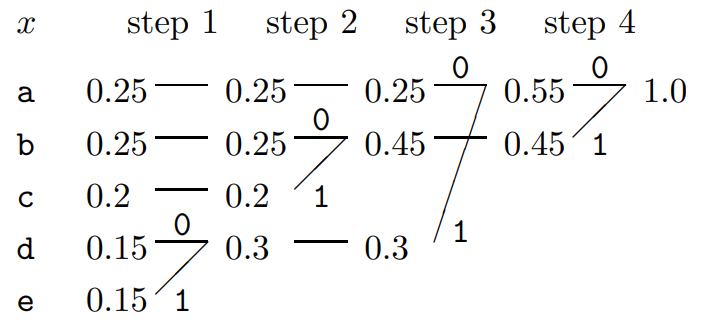
\includegraphics[width=1\textwidth]{images/huffman.png}
	\end{figure}
\end{minipage}
\begin{minipage}{0.50\textwidth}
	\begin{table}[H]
		\centering
		\renewcommand{\arraystretch}{1.55}
		\begin{tabular}{c|c|c|c|c}
			\hline
			$a_i$ & $p_i$ & $h(p_i)$ & $l_i$ & $c(a_i)$ \\
			\hline
			$a$ & 0.25 & 2.0 & 2 & 00 \\
			$b$ & 0.25 & 2.0 & 2 & 10 \\
			$c$ & 0.2 & 2.3 & 2 & 11 \\
			$d$ & 0.15 & 2.7 & 3 & 010 \\
			$d$ & 0.15 & 2.7 & 3 & 011 \\
			\hline
		\end{tabular}
	\end{table}
\end{minipage}

Calcoliamo l'entropia $H(X)$ e la lunghezza attesa $L(C,X)$
$$
H(X) = \frac{1}{4} \log_{2} 4 + \frac{1}{4} \log_{2} 4 + \frac{1}{5} \log_{2} 5 + \frac{3}{20} \log_{2} \frac{20}{3} + \frac{3}{20} \log_{2} \frac{20}{3} \approx 2,2855\ \text{bit}
$$
$$
L(C,X) = \frac{1}{4} \cdot 2 + \frac{1}{4} \cdot 2 + \frac{1}{5} \cdot 2 + \frac{3}{20} \cdot 3 +\frac{3}{20} \cdot 3 = 1 + \frac{2}{5} + \frac{9}{10} = \frac{23}{10} = 2,3\ \text{bit}
$$

\begin{center}
	\begin{tikzpicture}[scale=0.13]
		\tikzstyle{every node}+=[inner sep=0pt]
		\draw [black] (37.9,-10.4) circle (3);
		\draw (37.9,-10.4) node {$R$};
		\draw [black] (27.7,-19.9) circle (3);
		\draw (27.7,-19.9) node {$-$};
		\draw [black] (48,-19.9) circle (3);
		\draw (48,-19.9) node {$-$};
		\draw [black] (53.8,-28.7) circle (3);
		\draw (53.8,-28.7) node {$11$};
		\draw [black] (43.4,-28.7) circle (3);
		\draw (43.4,-28.7) node {$10$};
		\draw [black] (22.4,-28.7) circle (3);
		\draw (22.4,-28.7) node {$00$};
		\draw [black] (32.8,-28.7) circle (3);
		\draw (32.8,-28.7) node {$-$};
		\draw [black] (27.7,-38.5) circle (3);
		\draw (27.7,-38.5) node {$010$};
		\draw [black] (37.9,-38.5) circle (3);
		\draw (37.9,-38.5) node {$011$};
		\draw [black] (35.7,-12.44) -- (29.9,-17.86);
		\fill [black] (29.9,-17.86) -- (30.82,-17.68) -- (30.14,-16.94);
		\draw (31.78,-14.67) node [above] {$0$};
		\draw [black] (40.09,-12.46) -- (45.81,-17.84);
		\fill [black] (45.81,-17.84) -- (45.57,-16.93) -- (44.89,-17.66);
		\draw (43.97,-14.67) node [above] {$1$};
		\draw [black] (49.65,-22.4) -- (52.15,-26.2);
		\fill [black] (52.15,-26.2) -- (52.13,-25.25) -- (51.29,-25.8);
		\draw (51.51,-22.97) node [right] {$1$};
		\draw [black] (46.61,-22.56) -- (44.79,-26.04);
		\fill [black] (44.79,-26.04) -- (45.6,-25.56) -- (44.72,-25.1);
		\draw (45.02,-23.15) node [left] {$0$};
		\draw [black] (29.2,-22.5) -- (31.3,-26.1);
		\fill [black] (31.3,-26.1) -- (31.33,-25.16) -- (30.46,-25.66);
		\draw (30.9,-23.06) node [right] {$1$};
		\draw [black] (26.15,-22.47) -- (23.95,-26.13);
		\fill [black] (23.95,-26.13) -- (24.79,-25.7) -- (23.93,-25.19);
		\draw (24.41,-23.03) node [left] {$0$};
		\draw [black] (31.42,-31.36) -- (29.08,-35.84);
		\fill [black] (29.08,-35.84) -- (29.9,-35.36) -- (29.01,-34.9);
		\draw (29.56,-32.46) node [left] {$0$};
		\draw [black] (34.18,-31.36) -- (36.52,-35.84);
		\fill [black] (36.52,-35.84) -- (36.59,-34.9) -- (35.7,-35.36);
		\draw (36.04,-32.46) node [right] {$1$};
	\end{tikzpicture}
\end{center}


La codifica ottenuta è: $C=\{00, 10, 11, 010, 011\}$

\subsubsection{Svantaggi della Codifica di Huffman}
La codifica di Huffman produce un codice simbolico ottimo per una variabile aleatoria $X$, ma non è esente da difetti:
\begin{enumerate}
	\item \textbf{Cambio di variabile aleatoria}: I codici Huffman non possono gestire in modo efficiente il cambio di probabilità di una v.a. e si è costretti a ricreare un nuovo codice di Huffman o ad usare altri approcci \textbf{sotto-ottimali}.
	\item \textbf{Extra-bit}: I codici di Huffman, seppur ottimi, possono produrre un overhead di un extra bit per simbolo. Se l'entropia $H(X)$ è grande, questo overhead è trascurabile, ma se l'entropia $H(X)$ è di un bit per simbolo (o anche minore), l'overhead $L(C,X) - H(X)$ potrebbe dominare la lunghezza del file	codificato. 
\end{enumerate}


\newpage

\chapter{Comunicazione su canali Rumorosi}
Abbiamo parlato già all'inizio del capitolo di un esempio di canale rumoroso e di alcuni semplici tecniche di rilevamento e correzione degli errori. Essendo i \textbf{canali reali rumorosi}, il nostro obiettivo è esaminare se è possibile usare un canale rumoroso per comunicare in modo \textbf{affidabile}.

\section{Canali Rumorosi}
\paragraph{Definizione di Canale discreto memoryless}
Un \textbf{canale discreto memoryless} $Q$ è caratterizzato da un alfabeto di \textbf{input} $A_X$, un alfabeto di \textbf{output} $A_Y$ e un insieme di distribuzioni di probabilità $Pr[y|x]$, ognuna per ogni $x\in A_X$.\\
Queste probabilità di transizione possono essere memorizzate in una matrice:
\begin{equation}
	Q_{j|i} = Pr[y = b_j | x = a_i] \qquad 
	\begin{cases}
		\text{j-esima riga} \\
		\text{i-esima colonna}
	\end{cases}
\end{equation}

\subsubsection{Definizione di capacità di canale}
La capacità di un canale $Q$ definisce la massima mutua informazione:
\begin{equation}
	C(Q) = \max_{P_X}\ I(X;Y)
\end{equation}

La distribuzione $P_X$ per cui ottieniamo il massimo di $I(X;Y)$ è chiamata \textbf{distribuzione input ottimale}.


\subsection{Esempi di canali rumorosi}
\textbf{Canale Binario Simmetrico}:

Dati $A_X = \{0,1\}$  e $A_Y = \{0,1\}$ abbiamo:\\
\begin{minipage}{0.25\textwidth}
	\begin{figure}[H]
		\centering
		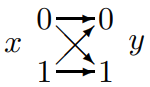
\includegraphics[width=0.7\textwidth]{images/cbs.png}
	\end{figure}
\end{minipage}
\begin{minipage}{0.50\textwidth}
	$$
	P(y = 0|x= 0) = 1 -f;\quad P(y = 0| x=1) = f;
	$$
	$$
	P(y=1|x=0) = f;\quad P(y=1|x=1) = 1 - f;
	$$
\end{minipage}
\begin{minipage}{0.25\textwidth}
	\begin{figure}[H]
		\centering
		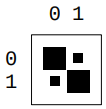
\includegraphics[width=0.5\textwidth]{images/prCbs.png}
	\end{figure}
\end{minipage}

\textbf{Z-Channel}:

Dati $A_X = \{0,1\}$  e $A_Y = \{0,1\}$ abbiamo:\\
\begin{minipage}{0.25\textwidth}
	\begin{figure}[H]
		\centering
		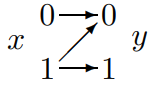
\includegraphics[width=0.7\textwidth]{images/zchan.png}
	\end{figure}
\end{minipage}
\begin{minipage}{0.50\textwidth}
	$$
	P(y = 0|x= 0) = 1;\quad P(y = 0| x=1) = f;
	$$
	$$
	P(y=1|x=0) = 0;\quad P(y=1|x=1) = 1 - f;
	$$
\end{minipage}
\begin{minipage}{0.25\textwidth}
	\begin{figure}[H]
		\centering
		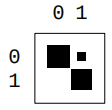
\includegraphics[width=0.5\textwidth]{images/prZchan.png}
	\end{figure}
\end{minipage}

\textbf{Noisy Typewriter}:

Dati $A_X = A_Y = \{\verb|A|, \verb|B|, \verb|C|, \cdots, \verb|Z|, \verb|-|\}$. Le 27 lettere sono raggruppate in un cerchio e quando il dattilografo (typist) prova a scrivere (ad esempio) \verb|B|, il risultato può essere \verb|A,B| o \verb|C|, con ognuno probabilità $\frac{1}{3}$.\\
La lettera finale '\verb|-|' simboleggia la lettera \verb|A|\\
\begin{minipage}{0.20\textwidth}
	\begin{figure}[H]
		\centering
		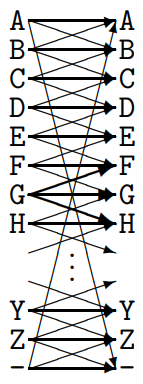
\includegraphics[width=0.6\textwidth]{images/ntype.png}
	\end{figure}
\end{minipage}
\begin{minipage}{0.50\textwidth}
	$$
	Pr(y = A|x= B) = \frac{1}{3}
	$$
	$$
	Pr(y = B|x= B) = \frac{1}{3}
	$$
	$$
	Pr(y = C|x= B) = \frac{1}{3}
	$$
\end{minipage}
\begin{minipage}{0.25\textwidth}
	\begin{figure}[H]
		\centering
		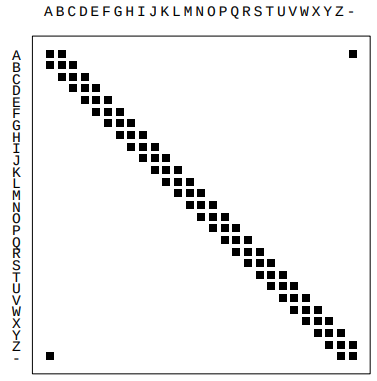
\includegraphics[width=1.2\textwidth]{images/prNtype.png}
	\end{figure}
\end{minipage}

\newpage
\textbf{Esempio N.1 - Mutua Informazione su Canale Binario Simmetrico}

Supponiamo che $f=0.15$ e che $P_X = \{p_0 = 0.9\ , p_1 = 0.1\}$. Calcoliamo $I(X;Y)$

Innanzitutto calcoliamo $Pr[y=0]$ e $Pr[y=1]$.
$$
Pr[y=0] = Pr[y=0|x=0]\cdot Pr[x=0] + Pr[y=0|x=1]\cdot Pr[x=1] = (1-f)\cdot p_0 + f\cdot p_1 = 
$$
$$
0.85 \cdot 0.9 + 0.15 \cdot 0.1 = 0.78
$$
$$
Pr[y=1] = Pr[y=1|x=0]\cdot Pr[x=0] + Pr[y=1|x=1]\cdot Pr[x=1] = f\cdot (1- p_0) + (1-f)\cdot p_1 = 
$$
$$
0.15 \cdot 0.9 + 0.85 \cdot 0.1 = 0.22
$$

Per calcolare $I(X;Y) = H(Y) - H(Y|X)$, devo prima calcolare $H(Y)$ e $H(Y|X)$. Cominciamo con $H(Y)$:
$$
H(Y) = - Pr[y=0] \log_2 Pr[y=0] + Pr[y=1] \log_{2} Pr[y=1] =
$$
$$
= \left(0.78 \cdot \log_2 (0.78) + 0.22 \cdot \log_2 (0.22) \right) = H(Pr[y=1]) = H(0.22) = 0.76
$$

Prima di calcolare $H(Y|X)$ dobbiamo ricavare $H(Y|x=0)$ e $H(Y|x=1)$. Cominciamo con $H(Y|x=0)$:
$$
H(Y|x=0) = Pr[y=0|x=0] \log_2 (Pr[y=0|x=0]) + Pr[y=1|x=0] \log_2 (Pr[y=1|x=0]) =
$$
$$
= (1-f)\log_2 (1-f) + f \log_2 f = H(f)
$$

Adesso calcoliamo $H(Y|x=1)$:
$$
H(Y|x=1) = Pr[y=0|x=1] \log_2 (Pr[y=0|x=1]) + Pr[y=1|x=1] \log_2 (Pr[y=1|x=1]) =
$$
$$
= f \log_2 f + (1-f)\log_2 (1-f) = H(f)
$$

Infine calcoliamo $H(Y|X)$:
$$
-\sum_{x\in X}\sum_{y\in Y} Pr[X=x,\ Y=y]\ \log_2 (Pr[Y=y|X=x]) = \sum_{x\in X} Pr[X=x] H(Y|X=x) = 
$$
$$
= p_0\ H(Y|x=0) + p_1 H(Y|x=1) = 0.9\ H(f) + 0.1\ H(f) = H(f) = H(0.15) = 0.61
$$

Calcoliamo la Mutua Informazione:
$$
I(X;Y) = H(0.22) - H(0.15) = 0.76 - 0.61 = 0.15\ \text{bit}
$$

\textbf{Possiamo fare meglio di così? Si, infatti calcolando la capacità di canale}:
$$
C(Q_{BSC}) = H(0.5) - H(0.15) = 1.0 - 0.61 = 0.39\ \text{bit}
$$

\begin{figure}[h]
	\centering
	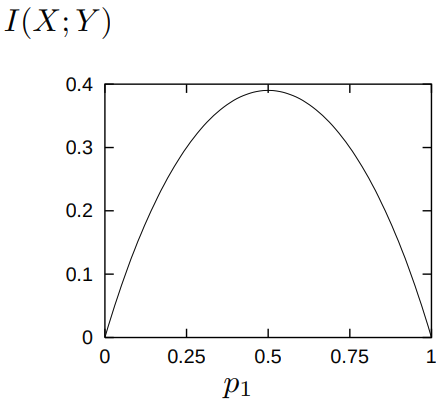
\includegraphics[width=0.5\textwidth]{images/QCBS}
\end{figure}

\newpage

\textbf{Esempio N.2 - Mutua Informazione su Z-Channel}

Supponiamo che $f=0.15$ e che $P_X = \{p_0 = 0.9\ , p_1 = 0.1\}$. Dobbiamo ricavare $I(X;Y)$
$$
H(Y) = H(Pr[y=1]) = H((1-f)\cdot p_1) = 0.42
$$
$$
Pr[y=0] = Pr[y=0|x=0]\cdot Pr[x=0] + Pr[y=0|x=1]\cdot Pr[x=1] =
$$
$$
0 + (1-f)\cdot p_1 = 0.85\cdot 0.1 = 0.085
$$
Calcoliamo $H(Y|X)$:
$$
H(Y|X) = H(Y|x=0)\ Pr[x=0] + H(Y|x=1)\ Pr[x=1] =
$$
$$
H(Pr[y=1|x=0])\ p_0 + H(Pr[y=1|x=1])\ p_1 = 0 + H(1-f)p_1 = H(0.85) \cdot 0.1 = 0.61 \cdot 0.1 = 0.061
$$
Adesso calcoliamo $I(X;Y)$
$$
I(X;Y) = H((1-f)\cdot p_1) - p_1\cdot H(1-f) = 0.42 - 0.061 = 0.36\ \text{bit}
$$

Questa funzione in $p_1^* = 0.445$ con $f=0.15$ non è banale.
La capacità di canale $C(Q_Z) = 0.685\ \text{bit}$

\begin{figure}[h]
	\centering
	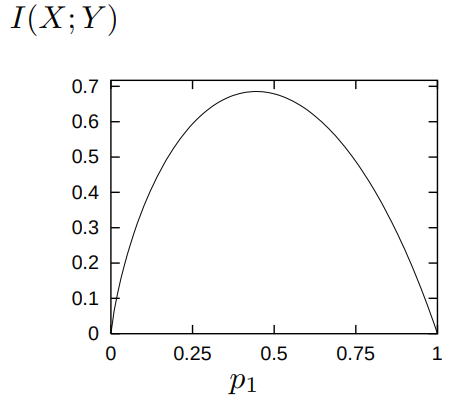
\includegraphics[width=0.5\textwidth]{images/QZchan}
\end{figure}

\textbf{Esempio N.3 - Capacità del Noisy Typewriter Channel}

Si trova che la distribuzione ottimale input è la distribuzione uniforme che dà:
$$
C(Q_{NT}) = \log_{2} 9 = 3,17\ \text{bit}
$$

\subsection{Teorema del Codice di un Canale Rumoroso}
La capacità di canale misura la frequenza di quanti \textbf{blocchi di informazione} possono essere trasferiti nel canale con una \textit{piccola quantità di errore arbitraria}.

\subsubsection{$(N,K)$ codici a blocco}
Un $(N,K)$ codice a blocco per un canale $Q$ è una lista di $S=2^K$ codeword tali che:
\begin{equation}
	{x^{(1)}, x^{(2)}, \cdots, x^{(2^K)}}, \quad x^{(s)}\in A_X^N
\end{equation}
ognuna con lunghezza $N$. Ci permette di codificare $S = 2^K$ segnali usando blocchi di lunghezza $N$.

\textit{OSSERVAZIONE}: Il numero di codewords $S$ è un intero, ma il numero di bit necessario per scegliere una codeword, ovvero $K\equiv \log_2 S$, non è necessariamente un intero.

\newpage
\subsubsection{Tasso di comunicazione}
Il tasso di comunicazione del codice per canale è:
\begin{equation}
	R = \frac{K}{N}\ \text{bit}
\end{equation}

\textit{OSSERVAZIONE}: Questa definizione è usata per qualsiasi canale, tuttavia se il canale non ha un alfabeto di input binario e contiene $q$ simboli, il tasso di comunicazione diventa:
\begin{equation}
	R = \frac{K}{N \log_{2} q}\ \text{bit} 
\end{equation}

\subsubsection{Decoder per $(N,k)$ codici a blocco}
Un decoder per $(N,k)$ codici a blocco mappa da un insieme di stringhe di output $S$ di lunghezza $N$, ovvero $A_Y^N$, un segnale $$\hat{s} \in \{0,1,2,\cdots,2^K\}$$

\textit{OSSERVAZIONE}: Il simbolo $\hat{s} = 0$ può essere usato per indicare un \textbf{fallimento}.

\subsubsection{Probabilità di un errore di blocco}
La \textbf{probabilità di un errore di blocco} di un codice e di un decoder, dato un canale e una distribuzione di probabilità sul segnale codificato $P(s_{in})$ è:
\begin{equation}
	p_B = \sum_{s_{in}} P(s_{in})\cdot P(s_{out} \neq s_{in}|s_{in})
\end{equation}

\subsubsection{Probabilità massima di un errore di blocco}
La probabilità \textbf{massima} di un errore di blocco è:
\begin{equation}
	p_{BM} = \max_{s_{in}} P(s_{out} \neq s_{in}|s_{in})
\end{equation}

\subsubsection{Probabilità di errore di bit}
Assumendo che $s$ sia rappresentato da un da un vettore binario \textbf{s} di lunghezza $K$, la probabilità di bit error consiste nella probabilità media che che un bit dell’output sia
diverso dal corrispondente bit dell’input.
\begin{equation}
	p_b = \max_{s} \left(\frac{1}{k} \sum_{i=1}^{k} Pr[\hat{s}(i) \neq s(i)|s]\right)
\end{equation}

\subsubsection{Decoder Ottimale}
Il decoder ottimale per un dato canale è quello che minimizza la probabilità di \textbf{errore di blocco}.\\ 
Decodifica un output $y$ come $\hat{s}$ che ha la massima probabilità a posteriori:
\begin{equation}
	p[s|y] = \frac{[y|s]\cdot p[s]}{\sum_{s'_{\text{input}}} P(y|s')\cdot P(s')}
\end{equation}

con: $\hat{s_{\text{output}}} = \text{argmax}\ P(s|y)$
\newpage
\subsection{Teorema di Shannon per canali rumorosi}
Il Teorema di compone di tre parti:
\begin{enumerate}
	\item Per ogni canale discreto di tipo \textbf{memoryless}, la capacità di canale:
	\begin{equation}
		C = \max_{P_X} I(X;Y)
	\end{equation}
	ha la seguente proprietà. Per ogni $\varepsilon > 0$, $R < C$ ed $N$ sufficientemente grande, esiste un codice di lunghezza $N$ e tasso $\geq R$ ed un decoder tale che la probabilità di block error massima è $< \varepsilon$.
	
	\item Se si ammette una probabilità di bit error $p_b$, tassi fino a
	\begin{equation}
		R(p_b) = \frac{C}{1 - H_2(p_b)}
	\end{equation}
	\textbf{sono possibili}.
	
	\item Per ogni $p_b$ tassi maggiori di $R(p_b)$ \textbf{non sono possibili}.
\end{enumerate}

\subsubsection{Conferma del Teorema di Shannon per canali rumorosi sul Noisy Typewriter Channel}

Possiamo creare una strategia di comunicazione completamente \textbf{priva di errori} usando un codice a blocchi di lunghezza $N=1$.\\ Usiamo come alfabeto un sottoinsieme di $A_X$ formato dalle lettere ogni 3: \verb|B,E,H,|$\cdots$\verb|,Z| 

Ognuno di questi simboli può essere \textbf{univocamente decodificato} scegliendo la decodifica come il simbolo più vicino di $A_X$. Questo sottoinsieme d'input ha 9 elementi e il tasso di comunicazione è uguale alla capacità del canale NT:
$$
Q(C_{NT}) = \log_2 9
$$

\begin{figure}[h]
	\centering
	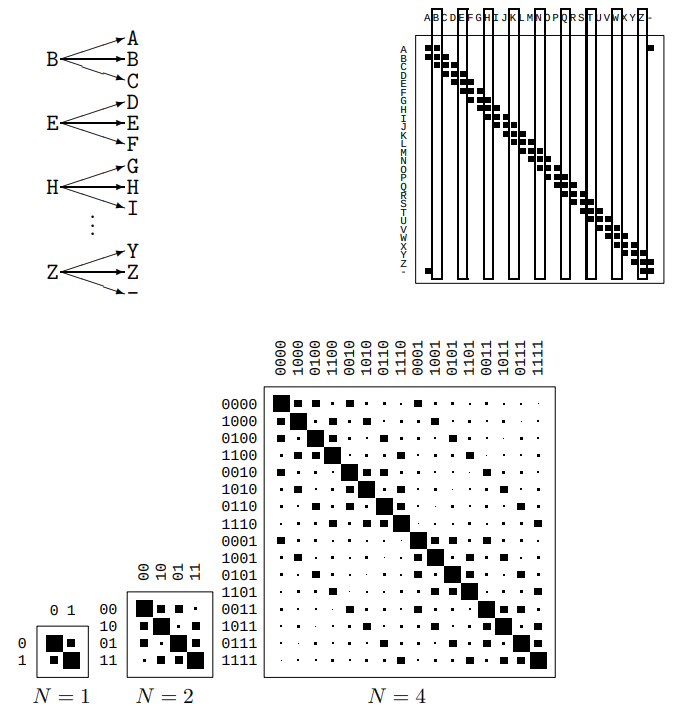
\includegraphics[width=0.8\textwidth]{images/proofNT.png}
\end{figure}



\include{./chapters/classica6}
\include{./chapters/classica7}
\include{./chapters/classica8}

\part{Informazione Quantistica}

\chapter{Fondamenti di Algebra Lineare}
\section{Algebra Lineare}
Consideriamo lo \textbf{spazio di Hilbert} $\mathbb{C}^d$ dei vettori colonna sui numeri complessi:
$$
v =
\begin{pmatrix}
  v_1 \\
  v_2 \\
  \vdots \\
  v_d
\end{pmatrix},
\hspace{0.3cm} v_i \in \mathbb{C}
$$
Dotato del prodotto scalare $\braket{v|w} = \sum^{d-1}_{i=0}\bar{v_i}w_i$.
Se $\mathcal{H}$ è uno spazio di Hilbert arbitrario con $\dim(\mathcal{H} = d)$ finita, posso scegliere una \textit{Base ortonormale} $\left\{ \ket{e_i} \right\}^d_{i=1}$ di $\mathcal{H}$, cioè t.c
$$\braket{e_i|e_j} 
\begin{cases}
 \hspace{0.2cm}1 \hspace{0.8cm} i=j \\
 \hspace{0.2cm}0 \hspace{0.8cm} i\neq j
\end{cases}
$$
Indichiamo i vettori di $\mathcal{H}$ con il simbolo $\ket{\Psi}$ e $\bra{\psi}$ per il suo duale,\\
\textbf{Base Ortonormale standard} di $\mathcal{H} = \mathbb{C}^d$
$$
\ket{0}=
\begin{pmatrix}
    1 \\
    0 \\
    \vdots \\
    0
\end{pmatrix}, 
\ket{1}=
\begin{pmatrix}
    0 \\
    1 \\
    \vdots \\
    0
\end{pmatrix}, \dots,
\ket{d-1}=
\begin{pmatrix}
    0 \\
    0 \\
    \vdots \\
    1
\end{pmatrix}
$$

Se $\ket{\Psi} = 
\begin{pmatrix}
    \psi_1 \\
    \psi_2 \\
    \vdots \\
    \psi_{d-1}
\end{pmatrix}
$
allora: $$\ket{\Psi} = \sum^{d-1}_{i=0}\psi_i \ket{i} \qquad\text{e il suo duale è:}\quad \bra{\Psi} = \left(\bar{\psi_0},\bar{\psi_1},\dots,\bar{\psi}_{d-1} \right)$$

Il prodotto scalare soddisfa la \textbf{Disequazione di Schwartz}:
$$\forall \ket{\Phi},\ket{\Psi} \in \mathcal{H} = \mathbb{C}^d, \hspace{0.2cm} \left|\braket{\Phi|\Psi} \right|^2 \le \braket{\Phi|\Phi} \cdot \braket{\Psi|\Psi}$$
E vale solo se: $$\ket{\Phi} = k\ket{\Psi}, \exists k \in\mathbb{C}$$
 
La norma indotta del prodotto scalare è $\left| \left| \Psi\right| \right| = \sqrt{\braket{\Psi|\Psi}}$, per cui possiamo riscrivere il lemma di Schwartz come:
$$\braket{\Phi|\Psi} = \left| \left|\Phi \right| \right| \cdot \left| \left|\Psi \right| \right|$$
\newpage 
\subsection{Mappe lineari e matrici}
Utilizziamo funzioni lineari $f$, con le seguenti proprietà:
\begin{enumerate}
    \item $f(\lambda x) = \lambda f(x)$,
    \item $f(x+y) = f(x) + f(y)$ 
\end{enumerate}

Dati $\mathcal{H}= \mathbb{C}^d, \mathcal{K} = \mathbb{C}^e$ spazi di Hilbert, $\textit{lin}(\mathcal{H},\mathcal{K})$ è l'insieme delle \textbf{mappe lineari} da $\mathcal{H}$ a $\mathcal{K}$.\\ Se fissiamo una base per $\mathcal{H}$ e una base per $\mathcal{K}$ allora ogni mappa di $\textit{lin}(\mathcal{H},\mathcal{K})$ può essere scritta come una matrice $d\times e$
$$\textit{lin}(\mathcal{H},\mathcal{H}) = \textit{lin}(\mathcal{H}) \hspace{0.5cm} \mathbb{1} \text{ op. identità}$$
La \textbf{Traccia} di $M \in \textit{lin}(\mathcal{H})$ si calcola scegliendo una base $\Sigma$ di $\mathcal{H}$ e sommando gli elementi della diagonale principale.
$$\text{tr}[M] = \sum_{i \in \Sigma} \braket{i|M|i}$$
La traccia  è un invariante  per cambiamenti di base e soddisfa 
$$\text{tr}[MN] = \text{tr}[NM],\hspace{0.4cm} \forall M\in \textit{lin}(\mathcal{H,K}),N\in \textit{lin}(\mathcal{K,H})$$

Se $M\in \textit{lin}(\mathcal{H})$ e $N = \ket{\Psi}\bra{\Psi}$ per $\ket{\Psi}\in \mathcal{H}$ allora 
$\text{tr}[MN]=\braket{\Psi|M|\Psi}$

Se $M\in \textit{lin}(\mathcal{H})$ e $\exists\ket{\Psi}\in \mathcal{H}$ non nullo e $n \in \mathbb{C}$ t.c $M \ket{\Psi} = \lambda \ket{\Psi}$ allora $\ket{\Psi}$ è un \textbf{Autovettore} di $M$ con \textbf{Autovalore} $\lambda$.

Se $M\in \textit{lin}(\mathcal{H}_1,\mathcal{H}_2)$, dove $\mathcal{H}_1$ ha base $\Sigma_1$ e  $\mathcal{H}_2$ ha base $\Sigma_2$ allora 
$$M = \sum_{i \in \Sigma_1}\sum_{j \in \Sigma_2} M_{ij} \ket{i}\bra{j}\hspace{0.2cm} \text{e} \hspace{0.2cm} M_{ij} = \braket{i|M|j}$$
Sia  $M\in \textit{lin}(\mathcal{H}_1,\mathcal{H}_2)$, l'\textbf{Operatrore aggiuto} di $M$ è il \textit{"dagger"} di $M$
$$M^\dagger = \overline{M}^T$$
ed è tale che $$\braket{\Psi|M|\Phi} = \overline{\braket{\Phi|M^\dagger|\Psi}}$$

Ed inoltre
$$M^\dagger\in \textit{lin}(\mathcal{H}_2,\mathcal{H}_1) \qquad \text{e} \qquad M^\dagger = \sum_{i,j} \overline{M_{ij}} \cdot\ket{j}\bra{i}$$

$M\in \textit{lin}(\mathcal{H})$ è \textbf{Hermitiano} (o autoaggiunto) se $M = M^\dagger$, cioè significa che $M$ ha elementi diagonali $M_{ii}$ reali e $M_{ij} = \overline{M_{ij}}$ per $i\neq j$.

$$\begin{pmatrix}
    1 & 1+i \\
    1-i & 0\\
\end{pmatrix}$$
Le matrici Hermitiane hanno autovalori reali e ammettono una base di autovettori.
\subsubsection{Teorema Spettrale}
Sia $M\in \textit{lin}(\mathcal{H})$ Hermitiana e $\dim (\mathcal{H} = d)$, allora 
$\exists \lambda_1\ge\lambda_2\ge\dots\ge \lambda_d \in \mathbb{R}$ e una base $\left\{\ket{\Psi}\right\} ^d_{i=1} $ t.c.
$$M = \sum^d_{i=1}\lambda_i \ket{\Psi_i}\bra{\Psi_i}\hspace{0.4cm} \text{e\hspace{0.4cm} $\left\{ \lambda\right\} ^d_{i=1} $ si chiama \textbf{Spettro di M}}$$

Questo teorema ci dice che una matrice hermitiana può essere diagonalizzata usando matrici unitarie e la matrice diagonale ha elementi reali.
\medskip
\\OSS: lo spettro è univocamente è univocamente determinato da $M$ ma gli autovalori potrebbero essere non unici se lo spettro è degenere.
\\esempio: $\mathbb{1} = \sum^d_{i=1}\ket{\Psi_i}\bra{\Psi_i}, \hspace{0.2cm} \forall \left\{ \ket{\Psi_i}\right\} ^d_{i=1}$ 

\medskip
Se $M$ è Hermitiano  (o unitario) e $f$ è una funzione a una variabile, allora
$$f(M) = \sum^d_{i=1} f(\lambda_i)\ket{\Psi_i} \bra{\Psi_i}$$
Ossia: bisogna che $f$ sia ben definita sullo spettro.

\subsubsection{Operatori Positivi}
$P \in \textit{lin}(\mathcal{H})$ è \textbf{Semidefinito positivo} (\textit{PSD}) oppure solo \textit{positivo} se
$$\forall \ket{\Psi} \in \mathcal{H}, \braket{\Psi|P|\Psi} \ge 0$$
\textbf{PSD($\mathcal{H})$} è l'insieme degli operatori $P\ge 0$ su $\mathcal{H}$
\medskip

$P \in \textit{lin}(\mathcal{H})$ è \textbf{Definitivo positivo} (\textit{PD}) $P > 0$ se $\forall \braket{\Psi|P| \Psi} > 0$

\medskip
\textit{PD($\mathcal{H}$)} è l'insieme degli operatori $P > 0$ su $\mathcal{H}$

\medskip 
\textbf{Lemma (caratterizzazione degli operatori PSD)}:

$P \in \textit{lin}(\mathcal{H})$ equivale a dire:
\begin{itemize}
    \item[\textbf{A.}] $P$ è \textit{PSD}, $\braket{\Psi|P|\Psi} \ge 0 \hspace{0.5cm} \forall\ket{\Psi}\in\mathcal{H}$ 
    \item[\textbf{B.}] $P$ è Hermitiano e i suoi autovalori sono \textbf{non negativi}
    \item[\textbf{C.}] $\exists M \in \textit{lin}(\mathcal{H,K}):P=M^\dagger M \hspace{0.3cm} \exists \mathcal{K}$ spazio di Hilbert
    \item[\textbf{D.}] $\forall Q \in PSD(\mathcal{H}),\  \text{tr}[PQ] \ge 0$
\end{itemize}

\subsubsection{Corollario}
Se $$P \in PSD(\mathcal{H}), M \in \textit{lin}(\mathcal{H,K})$$ allora $$MPM^\dagger \in PSD(\mathcal{K}) \qquad P\le Q \Leftrightarrow Q-P \ge 0$$
Questa nozione induce un ordinamento...

\subsubsection{Matrici Unitarie e Isometrie}
\begin{itemize}
	\item $V \in \textit{lin}(\mathcal{H,K})$ è \textbf{Isometria} se $V^\dagger V = \mathbb{1}$ (solo se $\dim(\mathcal{H}) \le\dim(\mathcal{K})$)
	
	\item $V\in \textit{lin}(\mathcal{H})$ è \textbf{Unitaria} se $U^\dagger U = UU^\dagger = \mathbb{1}$
	
\end{itemize}

Definiamo $U(\mathcal{H})$ l'\textbf{insieme delle matrici unitarie} su $\mathcal{H}$:
$$\textit{Isom}(\mathcal{H,K})$$ 
insieme delle matrici isometrie da $\mathcal{H}$ a $\mathcal{K}$

$P \in \textit{lin}(\mathcal{H})$ è una \textbf{Proiezione} se $P^2 = P$ e $P$ è Hermitiana.

Sia $$\left\{\ket{e_i} \right\}^d_{i=1}$$ base per l'immagine di una proiezione $P$, allora 
$$P = \sum^d_{i=1}\ket{e_i}\bra{e_i}$$

Supponiamo $M$ Hermitiana, allora $M = \sum^d_{i=1} \lambda_i \ket{\Psi_i}\bra{\Psi_i}$

\medskip
I proiettori sono $P_\lambda = \sum_{i=\lambda} \ket{\Psi_i}\bra{\Psi_i}$

\medskip
Se $\Lambda =$ insieme degli autovalori \underline{distinti}, allora $$M = \sum_{\lambda\in \Lambda} \lambda P_\lambda$$

In generale $$M\in\textit{lin}(\mathcal{H,K}) \quad \text{,} \quad M = \sum^r_{i=1} s_i\ket{e_i}\bra{f_i}$$
con $s_i\ge0$ autovalori, $r = \textit{rank}(M)$ ed $e_i,f_i$ basi di $\mathcal{H}$ e $\mathcal{K}$.

\newpage
\subsection{Prodotti tensoriali}
Def. $\mathcal{H,K}$ spazi di Hilbert, il loro \textbf{Prodotto tensoriale $\mathcal{H} \otimes \mathcal{K}$} è lo spazio di Hilbert che contiene tutte le combinazioni lineari di vettori della forma $v \otimes u, \hspace{0.2cm} v\in\mathcal{H}, w \in \mathcal{K}$
\begin{itemize}
    \item $(\alpha v) \otimes (\beta w) = \alpha\beta \cdot v\otimes w, \hspace{0.2cm} \forall\alpha,\beta \in \mathbb{C}$
    \item $(v_1 + v_2) \otimes w = v_1 \otimes w + v_2 \otimes w$
    \item $v + (w_1 \otimes w_2) = v \otimes w_1 + v \otimes w_2$
\end{itemize}
Il prodotto scalare è definito da
$$\braket{v_1 \otimes w_2 |v_2 \otimes w_2} = \braket{v_1|v_2} \otimes\braket{w_1|w_2}$$
Base di $\mathcal{H} \otimes \mathcal{K} \hspace{0.5cm} \left\{ \ket{i} \otimes\ket{j} \right\}, \ket{i}\in B_\mathcal{H}, \ket{j} \in B_\mathcal{K}$

\medskip
$\ket{\Phi}\ket{\Psi} = \ket{\Phi\Psi} = \ket{\Phi} \otimes \ket{\Psi}$

\medskip
$\ket{\Phi} ^{\otimes n} = \ket{\Phi} \otimes \dots \otimes \ket{\Phi} \hspace{0.5cm} \mathcal{H}^{\otimes n} = \mathcal{H} \otimes\dots\otimes\mathcal{H}$

\medskip
Se $M \in \textit{lin}(\mathcal{H}_1,\mathcal{H}_2)$ e $N \in \textit{lin}(\mathcal{K}_1,\mathcal{K}_2)$ allora
$$M\otimes N : \mathcal{H}_1 \otimes \mathcal{K}_1 \longrightarrow \mathcal{H}_2 \otimes \mathcal{K}_2 $$
$$(M \otimes N) (\ket{ \Phi} \otimes \ket{\Psi}) = M\ket{\Phi} \otimes N \ket{\Psi}$$
$$\textit{lin}(\mathcal{H}_1\otimes\mathcal{K}_1,\mathcal{H}_2\otimes\mathcal{K}_2) = \textit{lin}(\mathcal{H}_1,\mathcal{H}_2) \otimes \textit{lin}(\mathcal{K}_1,\mathcal{K}_2)$$
$$M = \sum_{i,j}M_{ij}\ket{i}\bra{j}, \quad N = \sum_{k,l} N_{kl} \ket{k}\bra{l}$$
$$M \otimes N = \sum_{i,j,k,l} M_{ij} N_{kl}\ket{i}\bra{j} \otimes \ket{k}\bra{l} = \sum_{i,j,k,l} M_{ij} N_{kl}\ket{ik}\bra{jl}$$

\textbf{Lemma 4.1}
\begin{description}
    \item[a.] $P \in \textit{PSD}(\mathcal{H}), Q \in \textit{PSD}(\mathcal{K}) \Rightarrow P \otimes Q \in \textit{PSD}(\mathcal{H}\otimes\mathcal{K})$
    \item[b.] $\forall M \in \textit{lin}(\mathcal{H}), N \in \textit{lin}(\mathcal{K}), \text{ tr}[M\otimes N] = \text{tr}[M]\text{tr}[N]$
    \item[c.] $\forall M \in \textit{lin}(\mathcal{H}), N \in \textit{lin}(\mathcal{K}), \text{ rank}(M\otimes N) = \text{rank}(M)\text{rank}(N)$
    \item[d.] $\ket{\Phi}\otimes z = z\ket{\Phi}, z \in \mathbb{C} \hspace{1cm}\mathcal{H} \otimes \mathbb{C}= \mathcal{H}$
    \item[e.] $M\otimes \ket{\Psi}: \mathcal{H} \longrightarrow \mathcal{H} \otimes \mathcal{K} \hspace{0.8cm} (M\otimes \ket{\Psi})\ket{\Phi} = M \ket{\Phi} \otimes \ket{\Psi}$
    
    \medskip
    $M\otimes \bra{\Psi}: \mathcal{H} \otimes \mathcal{K} \longrightarrow \mathcal{H} \hspace{0.8cm} (M\otimes \bra{\Psi}) (\ket{\Phi}\otimes\bra{\chi}) = \braket{\Psi|\chi} M \ket{\Phi} \otimes \in \mathcal{H}$
\end{description}

\section{Stati Quantistici}
$$\ket{0} = 
\begin{pmatrix}
    1 \\
    0 \\
\end{pmatrix}
\hspace{1cm}
\ket{1} = 
\begin{pmatrix}
    0 \\
    1 \\
\end{pmatrix}
$$
$$\ket{q} = \alpha\ket{0}+\beta\ket{1}=
\begin{pmatrix}
    \alpha \\
    \beta \\
\end{pmatrix}
\hspace{1cm} p(0)= \left|\alpha \right|^2, p(1)= \left|\beta \right|^2,\hspace{0.2cm} \left|\alpha \right|^2 +\left|\beta \right|^2 = 1
$$
\subsection{Spazi di Hilbert}
\textbf{Assioma 1:} Ogni sistema quantistico è associato ad uno spazio di Hilbert $\mathcal{H}$.

Se $\dim \mathcal{H} = d$ posso identificare $\mathcal{H}$ come $\mathbb{C}^d$ munito del prodotto scalare standard.
Un sistema quantistico associato a $\left(\mathbb{C}^d,<\cdot,\cdot> \right)= \mathcal{H}$ oìpuò essere pensato come avente $d$ possibili stati distinti.
\\Esempio: Lo spazio di Hilbert più banale è $\mathbb{C}^2$, associato ad un solo qubit , ed ha come base $\ket{0}$ e $\ket{1}$
\subsection{Stati Quantistici}
\textbf{Definizione Matrice Densità}: una \textbf{Matrice densità} è un operatore \textbf{semidefinito positivo}\\ $\rho \in \textit{PSD}(\mathcal{H})$ con traccia $\text{tr}[\rho]=1$.
Denotiamo l'insieme delle matrici densità su $\mathcal{H}$ con $$S(\mathcal{H})=\{\rho \in\textit{PSD}(\mathcal{H}:\text{tr}[\rho]=1\}$$

\textbf{Assioma 2}: Lo stato di un sistema quantistico con spazio di Hilbert $\mathcal{H}$ è descritto da una matrice densità.

\textbf{Stati classici}: Sia $\Omega$ un insieme di possibili risultati. Allora la collezione delle distribuzioni di probabilità su $\Omega$ è: $$P(\Omega)=\left\{p : \Omega\rightarrow\mathbb{R}_{\ge0}\quad|\quad\sum_{x \in \Omega}p(x)=1\right\}$$

Alcune volte $p_x:= p(x)$, inoltre $\left\{p_x \right\}_{x\in \Omega}$ è una distribuzione di probabilità.

Sia $\mathcal{H}$ spazio di Hilbert e supponiamo che $\left\{ \ket{x}:x \in \Omega \right\}$ sia una base di $\mathcal{H}$.
Allora possiamo associare ad ogni distrubuzione di probabilità $p \in P(\Omega)$ lo stato quantistico
$$\rho  = \sum_{x \in \Omega} p(x)\ket{x}\bra{x} \hspace{0.2cm} \in S(\mathcal{H})$$
Esempio: consideriamo la base standard dello spazio di Hilbert a un qubit, $\mathcal{H}= \mathbb{C}^2$ con base $\Omega = \{0,1\}$
$$\rho = p(0) \ket{0}\bra{0}+p(1) \ket{1}\bra{1}=
\begin{pmatrix}
    p(0) & 0\\
    0 & p(1) \\
\end{pmatrix}
$$
Analogamente, la base di $\mathcal{H} = \mathbb{C}^2$ è data da $\Omega = \{0,1,\dots,d-1\}$. (Nota: sost. i sigma con omega)

In generale se $\Omega$ è un insieme finito, scriviamo $\mathcal{H}= \mathbb{C}^d$ per denotare uno spazio di Hilbert ortonormale $\left\{ \ket{x}:x \in \Omega  \right\}$, i vettori di $\mathcal{H}$ sono combinazioni lineari \textit{"formali"} dei vettori della base
$$\mathcal{H} = \mathbb{C}^\Omega = \left\{ \ket{v} = \sum_{x\in \Omega} v_x \ket{x}:v_x \in \mathbb{C}\right\}$$
e il prodotto scalare è $\braket{v|w}=\sum_{x\in \Omega} \overline{v}_x w_x$

\medskip
\textbf{Definizione di Stato Classico}: Sia $\Omega$ un insieme finito. Uno stato quantistico $\rho \in S(\mathcal{H})$ su $\mathcal{H}= \mathbb{C}^\Omega$ è uno \textbf{Stato classico} se nella forma: $$\rho = \sum_{x\in \Omega}p(x)\ket{x}\bra{x}, \text{ con } p\in P(\Omega)$$
Esempio: Il lancio di una moneta: 
$$\rho = \frac{1}{2}\left( \ket{0} \bra{0}+ \ket{1}\bra{1}\right)= 
\frac{1}{2}
\begin{pmatrix}
    1 & 0\\
    0 & 1
\end{pmatrix}
$$
Gli stati classici sono matrici diagonali rispetto alla base computazionale.

\subsection{Stati Puri}
Dato $\ket{\Psi} \in \mathcal{H}$ con norma unitaria, ovviamente $||\ket{\Psi}|| = \braket{\Psi|\Psi}=1$ , non può essere associato alla matrice densità
$$\rho = \ket{\Psi} \bra{\Psi}$$

$\rho$ è una matrice densità, infatti $\rho \in$ PSD e tr$[\rho] = \text{tr}[\ket{\Psi}\bra{\Psi}]=\text{tr}[\braket{\Psi|\Psi}]=1$

%$\mathcal{H}$ (\textit{Lemma 0.2})

Definizione: uno \textbf{Stato puro} $\rho \in S(\mathcal{H})$ è tale se $\ket{\Psi} \in \mathcal{H}$ tale che $\rho = \ket{\Psi}\bra{\Psi}$. Uno stato non puro di dice \textbf{Stato Misto}.

C'è una ridondanza nella descrizione $\ket{\Psi}$ di uno stato (notazione di Dirac): moltiplicando per una fase globale la matrice densità \textbf{non cambia}. Sia $\ket{\Phi}= e^{i\theta}\ket{ \Phi}$ con $\Theta \in \mathbb{R}$, allora:
$$\ket{\Phi}\bra{\Phi} = (e^{i\theta}\ket{\Psi})(e^{i\theta}\bra{\Psi})^{\dagger} = 
e^{i\theta}\ket{ \Phi}e^{-i\theta}\bra{\Phi} = e^{i\theta-i\theta}\ket{ \Phi}\bra{\Phi}=
\ket{\Psi} \bra{\Psi}$$

\textbf{Lemma 1.3:} Sia $\rho\in S(\mathcal{H})$. Le seguenti condizioni sono equivalenti:
\begin{description}
    \item[a)] $\rho$ è uno stato puro
    \item[b)] $\rho$ ha rango 1
    \item[c)] $\rho$ è una proiezione
\end{description}

\textbf{Esempio}: In uno stato classico di dimensione 2 \textbf{non è puro}, la matrice densità sarà:
$$
\begin{pmatrix}
	\rho & 0\\
	0 & 1 - \rho
\end{pmatrix}
$$

Nel caso generale, sia $\ket{\psi}= \alpha\ket{0}+\beta\ket{1}$, con $\alpha, \beta \in \mathbb{C}$, $|\alpha|^2 + |\beta|^2=1$. Allora:
$$\rho= \ket{\psi}\bra{\psi}= 
\begin{pmatrix}
    \alpha \\
    \beta
\end{pmatrix}
\begin{pmatrix}
    \overline{\alpha} & \overline{\beta}
\end{pmatrix}
= \begin{pmatrix}
    \alpha^2 & \alpha\overline{\beta}\\
    \overline{\alpha}\beta & \beta^2
\end{pmatrix}
$$

\subsection{Stati quantistici generici}
Sia $\rho \in S(\mathcal{H}) \Rightarrow \rho \in \textit{PSD}(\mathcal{H}) \Rightarrow \rho$ è Hermitiana e i suoi autovalori sono non negativi, vale il \\\textbf{Teorema spettrale}:
$$\rho = \sum^d_{i=1}p_i \ket{\psi_i}\bra{\psi_i}$$
con $p_i\ge 0$ autovalori e $\left\{ \ket{\psi} \right\}^d_{i=1}$ base di autovettori.

Rispetto a questa base la matrice è diagonale e tr$[\rho] = \sum^d_{i=1} p_i = 1$
\\In altre parole gli autovalori $\left\{  p_i \right\}^d_{i=1}$ definiscono una distribuzione di probabilità: "abbiamo lo stato $\ket{ \Phi_i}$ con probabilità $\rho_i$".

%Interpretiamo lo stato $\rho$ come una situazione in cui abbiamo lo stato puro $\ket{\psi}$ con probabilità $p_i$.
\textbf{Osservazione}: Qualunque decomposizione $\rho = \sum^d_{i=1} p_i \ket{\psi_i}\bra{\psi_i}$ è simile alla nostra definizione di stato classico. La differenza cruciale è che per uno stato classico la matrice è diagonale rispetto alla base computazionale.
\medskip
\\Dato $\mathcal{H}$ di dimensione $d$ possiamo definire lo stato detto \textbf{Massimalmente Misto}: $$\tau_d=\frac{1}{d}\mathbb{1}$$
Questo stato può essere decomposto come:
$$\tau = \sum^d_{j=1} \frac{1}{d} \ket{e_j}\bra{e_j} \text{ di } \mathcal{H} \hspace{0.5cm} \left\{ \ket{e_j} \right\}^d_{j=1} \text{ base}$$
Ricordiamo che un insieme $X$ si dice \textbf{Convesso} se $\forall x_0,x_1 \in X$ e $\forall 0 \le t\le 1$, 
$$x_t = tx_1 + (1-t)x_0 \in X$$
Questo significa che tutti i punti del segmento tra $x_0$ e $x_1$ sono contenuti in $X$. Chiamiamo $x_t$ una \textbf{Combinazione Convessa} di $x_0$ e $x_1$. 

I \textbf{Punti estremi}, sono quelli che possono essere scritti solo come combinazioni banali ($t=0$ o $t=1$).

$P(\Sigma)$ è un insieme convesso che si chiama \textbf{Simplesso}. Dato un bit classico, $P(\{0,1\})$ è un segmento che congiunge $\begin{pmatrix}
    1 \\ 0
\end{pmatrix}
\text{ e }
\begin{pmatrix}
    0\\1
\end{pmatrix}
$, che sono due punti estremi.
\medskip
\\ \textbf{Lemma 1.6:} $S(\mathcal{H}) \subset \textit{lin}(\mathcal{H})$ è un insieme convesso e i suoi punti estremi coincidono con l'insieme dei suoi stati puri. 

\section{Qubit e Sfera di Bloch}
Le seguenti  matrici formano una base dello spazio vettoriale reale delle matrici hermitiane, sono dette \textbf{Matrici di Pauli}
$$
\mathbb{1}=
\begin{pmatrix}
    1 & 0\\
    0 & 1
\end{pmatrix}
, X =
\begin{pmatrix}
    0 & 1\\
    1 & 0
\end{pmatrix}
, Y=
\begin{pmatrix}
    0 & -i\\
    i & 0
\end{pmatrix}
, Z =
\begin{pmatrix}
    1 & 0 \\
    0 & -1
\end{pmatrix}
$$
\begin{itemize}
    \item $X,Y,Z$ hanno \textbf{Traccia 0} (\textit{traceless})
    \item Sono hermitiane e unitarie, pertanto $X^2=Y^2=Z^2=\mathbb{1}$
    \item $X,Y,Z$ hanno \textbf{Autovalori 1 e -1}
    \item $X,Y,Z$ si autocommutano e si semplificano ciclicamente
    $$XY = -YX, \hspace{0.2cm} YZ = -ZY,  \hspace{0.2cm} ZX = -XZ$$
    \item $X,Y,Z$ si moltiplicano ciclicamente:
    $$XY = iZ, \hspace{0.4cm} YZ = iX,  \hspace{0.4cm} ZX = iY$$ 
\end{itemize}
Anche la \textbf{traccia dei prodotti} ovviamente è uguale a 0.

Sia $\rho \in \textit{lin}(\mathbb{C^2})$ una matrice hermitiana arbitraria con tr$[\rho] = 1$
$$\rho = \frac{1}{2}\left( \mathbb{1} + xX + yY+zZ\right) = \frac{1}{2}
\begin{pmatrix}
    1+z & x-iy \\
    x+iy & 1-z
\end{pmatrix}, \quad \text{con}\  x,y,z\in \mathbb{R}$$
 
Siano $\lambda_1,\lambda_2 \in \mathbb{R}$ gli autovalori di $\rho$, allora $\lambda_1,\lambda_2 \ge 0$ e tr$[\rho]=1$
allora almeno uno tra $\lambda_1$ e $\lambda_2$ deve essere positivo. Quindi, $\rho \in \textit{PSD} \Leftrightarrow \lambda_1\lambda_2=\det(\rho)\ge0$
$$\det(\rho) = \frac{1}{4}\left( (1+z) (1-z) - (x-iy) (x+iy) \right) = \frac{1}{4}(1-x^2-y^2-z^2)$$
$$\rho \text{ è PSD } \Longleftrightarrow 1-x^2-y^2-z^2\ge 0 \Longleftrightarrow x^2+y^2+z^2 \le 1$$
$$ \Longleftrightarrow \vec{r}= (x,y,z) \text{ ha norma } ||\vec{r}|| \le1$$

Lo stato di un qubit è parametrizzato da una palla solida di raggio 1 ed è chiamata \textbf{Palla di Bloch} (\textit{Bloch Ball}), mentre il vettore $\vec{r}$ è chiamata \textbf{Vettore di Bloch}.

In che caso otteniamo uno stato puro? La risposta  viene data dal Lemma 1.2: se e solo se abbiamo un autovalore uguale a 1 e l'altro uguale a 0, così che $\det(\rho(\vec{r}))= 0$, il che è equivalente al fatto che $\vec{r}$ è unitario. Quindi gli stati puri di un qubit sono parametrizzati da una sfera unitaria su $\mathbb{R}^3$ chiamata \textbf{Sfera di Bloch}.

Lemma 2.1: Ogni $\rho \in S(\mathbb{C^2})$ di un qubit può essere scritto come
$$\rho = \frac{1}{2}\left( \mathbb{1} + xX + yY + zZ \right)$$
\begin{wrapfigure} {r}{0.35\textwidth}
    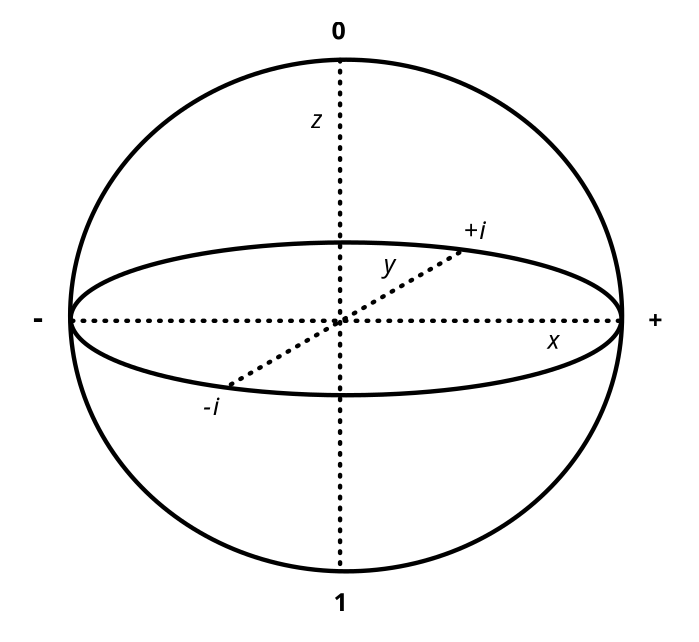
\includegraphics[width=1\linewidth]{images/Bloch.png}

\end{wrapfigure}
I punti interni rappresentano stati misti, in particolare il centro $\vec{r}=(0,0,0)$ corrisponde allo \textbf{Stato massimalmente misto} $$\rho(\vec{r})=\tau = \frac{\mathbb{1}}{2}$$
Un vettore $\vec{r}=(0,0,2p-1)$ sull'asse $\vec{z}$ con $p\in[0,1]$ corrisponde ad uno stato classico
$$\rho = \frac{1}{2}(\mathbb{1} + (zp-1)Z) = \frac{1}{2}
\begin{pmatrix}
    1+(2p-1) & 0\\
    0 & 1-(2p-1)
\end{pmatrix}
$$
$$
= \begin{pmatrix}
    p & 0\\
    0 & 1-p
\end{pmatrix}
$$
\newpage
Vediamo quali stati sono intersezione degli assi con la sfera:
\begin{itemize}
    \item Asse $\vec{z}$: \\$\vec{r}=(0,0,1)= \ket{0}$ , $\vec{r}=(0,0,-1)= \ket{1}$
    \item Asse $\vec{x}$: \\$\vec{r}=(1,0,0)= \ket{+}= \frac{1}{\sqrt{2}}(\ket{0} + \ket{1})$ , $\vec{r}=(-1,0,0)= \ket{- }= \frac{1}{\sqrt{2}}(\ket{0} - \ket{1})$
    \item Asse $\vec{y}$: \\$\vec{r}=(0,1,0)= \ket{+i}= \frac{1}{\sqrt{2}}(\ket{0} + i\ket{1})$ , $\vec{r}=(0,-1,0)= \ket{-i}= \frac{1}{\sqrt{2}}(\ket{0} - i\ket{1})$
\end{itemize}

Abbiamo ottenuto 3 diverse basi di $\mathbb{C^2}$, che chiamiamo basi $X,Y,Z$
\begin{itemize}
    \item I vettori della base $X$ sono gli autovettori $\ket{\pm}$ della matrice di Pauli $X$
    \item I vettori della base $Y$ sono gli autovettori $\ket{\pm i}$ della matrice di Pauli $Y$
    \item I vettori della base $Z$ sono gli autovettori $\ket{0},\ket{1}$ della matrice di Pauli $Z$
\end{itemize}

\section{Misurazioni}
Definizione: una \textbf{Misurazione} o \textbf{POVM} (\textit{Positive-Operator-Valued-Measure}) su uno spazio di Hilbert $\mathcal{H}$ con insieme dei risultati $\Omega$ è una collezione di operatori:
$$\mu=\left\{ \mu(x) \in \textit{PSD}(\mathcal{H}) \right\}_{x\in\Omega}\quad \text{tale che}\quad \sum_{x\in\Omega} \mu(x) = \mathbb{1}$$

Denotiamo con $\textit{Meas}(\mathcal{H},\Omega)$ l'insieme di tutte le misure su $\mathcal{H}$ con l'insieme dei risultati in $\Omega$, inoltre\\ $0\le\mu_x\le\mathbb{1}$ dove $\mu_x=\mu(x)$ 
(Notazione utilizzata) sono operatori che hanno autovalore $$\lambda:0\le\lambda\le1 \hspace{0.3cm} \forall x \in \Omega$$

\textbf{ASSIOMA 3 (Misurazioni)}

Quando eseguiamo una misurazione $\mu\in \textit{Meas}(\mathcal{H},\Omega)$ su uno stato quantistico $\rho\in S(\mathcal{H})$ osserviamo il risultato $x\in \Omega$ con probabilità $$p(x) = \text{tr}[\mu_x\rho]$$
Vediamo un esempio: con un singolo qubit consideriamo $\Omega= \{0,1\}$, e
$\mu=\{\mu_0,\mu_1\}:\mu_0=\ket{0}\bra{0},\mu_1=\ket{1}\bra{1}$, che definisce una misurazione. Misuriamo $\rho = \ket{\psi}\bra{\psi}$ per $\ket{\psi} = \ket{0}$

$$
    p(0)=\text{tr}[\mu_0\rho]=\text{tr}[\ket{0}\bra{0}\ket{0}\bra{0}] = 1
$$

$$
    p(1)=\text{tr}[\mu_1\rho]=\text{tr}[\ket{1}\bra{1}\ket{0}\bra{0}] = 0
$$

se invece $\ket{\psi} = \ket{+}$

$$
    p(0) = \text{tr}[\ket{0}\bra{0}\frac{1}{2}(\ket{0}+\ket{1})(\ket{0}+\ket{1})] = 
$$
$$
    = \frac{1}{2} \text{tr}\left[
    \begin{pmatrix}
        1 & 0\\
        0 & 0
    \end{pmatrix}
    \begin{pmatrix}
        1 & 1\\
        1 & 1
    \end{pmatrix}
    \right]
     = 
     \frac{1}{2} \text{tr}\left[
    \begin{pmatrix}
        1 & 0\\
        0 & 0
    \end{pmatrix}\right] = \frac{1}{2}
$$

analogamente $p(1) = \frac{1}{2}$.
\\Se consideriamo lo stato massimamente misto $\tau = \frac{1}{2}\mathbb{1}$
$$p(0)=\text{tr}[\ket{0}\bra{0}\frac{1}{2}\mathbb{1}] = \frac{1}{2}$$
e analogamente $p(1) = \frac{1}{2}$, cioè dalla misurazione non sappiamo distinguere $\ket{+}$ da $\tau$
\subsection{Misure rispetto a una base e misure proiettive}
Sia $\left\{\ket{e_x} \right\}_{x\in \Omega}$ una base arbitraria. Allora possiamo costruire una misurazione con l'insieme dei risultati $\Omega$, definendo
$$
    \mu_x = \ket{e_x}\bra{e_x} \hspace{0.3cm}\text{ per } x \in \Omega
$$
Quindi $\sum_{x\in\Omega}\mu_x = \sum_x \ket{e_x}\bra{e_x} = \mathbb{1}$ è una misura valida. Questo tipo di misura si chiama misura rispetto ad una base. In particolare, prendendo la base standard $\left\{ \ket{x} \right\}_{x\in\Sigma}$ otteniamo una misurazione rispetto alla base standard ($\Sigma$ insieme degli stati classici).
\medskip
\\ \textbf{Lemma 3.1} (\textit{Regola di Born}): Dato lo stato quantistico $\rho \in S(\mathcal{H})$, eseguendo una misura rispetto ad una base $\mu_x=\ket{e_x}\bra{e_x}$ osserviamo il risultato $x\in\Omega$ con probabilità $p(x)=\braket{e_x|\rho|e_x}$. Inoltre se $\rho = \ket{\psi}\bra{\psi}$ è uno stato puro $\ket{\psi}= \sum_{x\in\Omega}\Psi_x\ket{e_x}$ allora $p(x)=|\Psi_x|^2$
\medskip
\\ \textbf{Dimostrazione}: Poichè se $N = \ket{\psi}\bra{\psi}$ abbiamo che $$tr[MN]=\braket{\psi|M|\psi}$$ allora
$$p(x)= \text{tr}[\ket{e_x}\bra{e_x}\rho]=\braket{e_x|\rho|e_x}$$
Quando $$\rho = \ket{\psi}\bra{\psi}, \ket{\psi} = \sum_{x\in\Omega}\Psi_x\ket{\psi}$$ otteniamo $$p(x)=\braket{e_x|\psi} \braket{\psi|e_x}= |\braket{\psi|e_x}|^2=|\Psi|^2$$

Un caso più generale avviene quando gli operatori di misura $\mu_x$ sono tutte proiezioni, $\mu_x=P_x$. In tal caso abbiamo un operatore di misura proiettiva (\textit{PVM}). $\sum_{x\in\Omega}\mu_x = \mathbb{1}$, le immagini degli $\mu_x$ devono essere ortogonali e spannare tutto.
\subsection{Misurazione di qubit}
In generale scegliamo $\vec{r}=(x,y,z)$ con $||\vec{r}||=1$ e lo stato corrispettivo $-\vec{r}$. Allora 
$$\mu_{\vec{r},0}=p(\vec{r})=\frac{1}{2}
\begin{pmatrix}
    1+z & x-iy\\
    x+iy & 1-z
\end{pmatrix}\quad,\quad 
\mu_{-\vec{r},0}=p(-\vec{r})=\frac{1}{2}
\begin{pmatrix}
    1-z & -x+iy\\
    -x-iy & 1+z
\end{pmatrix}
$$
Se eseguiamo questa misura su uno stato quantistico con vettore di Bloch $\vec{s}=(x',y',z')$ allora la probabilità di ottenere $0$ è: $$p(0)= \frac{1}{2}+\frac{1}{2}\vec{r}\cdot\vec{s}=\frac{1}{2}+\frac{1}{2}(xx'+yy'+zz')$$ 

Geometricamente, $\vec{r}\cdot\vec{s}$ è la proiezione del vettore del Bloch...

Non esiste alcuno stato quantistico per cui entrambe le misure $X$ e $Z$ sono certe. Le misurazioni mappano uno stato quantistico in uno stato classico.

\textbf{Lemma 3.2}: Dato $\Omega$ insieme dei risultati classici, $\mathcal{H}$ spazio di Hilbert, supponiamo che per ogni $\rho\in S(\mathcal{H})$ esista una distribuzione di probabilità:
$$P_\rho\in P(\Omega): p\rho =p_1\rho_1+p_2\rho_2$$ per ogni stato misto
$\rho = p_1\rho_1+p_2\rho_2$. 

Allora, esiste un operatore di misura: $$\mu:\Omega\rightarrow\textit{PSD}(\mathcal{H}):\forall x\in\Omega, p\rho(x)=\textit{tr}[\mu(x)\rho]$$

\newpage
\section{Sistemi quantistici multipli}
Se $\mathcal{H}$ ha una base indicizzata $\ket{x_j}$ da $\ket{x_j}\in \Sigma_j$, allora il prodotto tensoriale $\mathcal{H}_1\otimes\mathcal{H}_2\otimes\dots\otimes\mathcal{H}_n$ ha la base prodotto $\ket{x_1,x_2,\dots,x_n}=\ket{x_1}\ket\otimes{x_2}\otimes\dots\otimes\ket{x_n}$
\medskip
\\ \textbf{ASSIOMA 4 (Sistemi multipli)}
\\Se abbiamo n sistemi quantistici con rispettivi spazi di hilbert $\mathcal{H}_1,\mathcal{H}_2,\dots,\mathcal{H}_n$, allora il sistema congiunto è associato allo spazio di Hilbert $\mathcal{H}_1\otimes\mathcal{H}_2\otimes\dots\otimes\mathcal{H}_n$
\medskip
\\ \textit{Notazione:} $A,B,C $ :Sistemi, $\hspace{0.5cm}\mathcal{H}_A,\mathcal{H}_B,\mathcal{H}_C$ : Spazi associati
\medskip
\\ $\rho_A,\rho_B,\rho_C,\rho_{AB},\rho_{BC},\rho_{AC},\rho_{ABC}$: Stati cogiuti
\medskip
\\$\Sigma_A,\Sigma_B,\Sigma_C$: Alfabeti di simboli
\medskip
\\ $\textit{lin}(A)= \textit{lin}(\mathcal{H}_A)$, $\hspace{0.3cm}S(A) = S(\mathcal{H}_A)$, $\hspace{0.3cm}\textit{PSD}(A)= \textit{PSD}(\mathcal{H}_A)$
\medskip
\\ $\mu_A\in\textit{Meas}(\mathcal{H}_A,\Omega)$, $\hspace{0.5cm}\Sigma_{AB}= \Sigma_A\times\Sigma_B$
\medskip
\\ \textit{Defizione}: $A,B$ stati quabtistici. Gli stati  nella forma $\rho=\rho_A\otimes\rho_B,\rho_A\in S(A),\rho_B\in S(B)$ si chiama \textbf{Stato prodotto}. Uno stato che non è prodotto si dice \textbf{Stato correlato}.
\\Se abbiamo $N$ sistemi, $\rho_{A_1,\dots,A_n}\in S(A_1,\dots,A_n)$ è uno stato prodotto se $\rho_{A_1,\dots,A_n}=\rho_{A_1}\otimes\dots\otimes\rho_{A_n},\hspace{0.3cm}\rho_{A_i}\in S(A_i)$

\textbf{Esempio}: Alice e Bob hanno un qubit ciascuno,   $\mathcal{H}_A = \mathcal{H}_b = \mathbb{C}^2 \ \Rightarrow\  \mathcal{H}_A\otimes\mathcal{H}_B \cong
\mathbb{C}^4$
\begin{enumerate}
    \item Essi potrebbero condividere uno degli stati base: $\ket{00},\ket{01},\ket{10},\ket{11}$, che corrispondono a stati puri e classici;
    \item Potrebbero avere $\ket{+}_A\ket{+}_B= \frac{1}{2}\left( \ket{00}+\ket{01}+\ket{10}+\ket{11} \right)$, che corrisponde ad uno stato \textbf{puro} ma non classico;
    \item Uno stato classico \textbf{non prodotto} si dice \textbf{Massimamente correlato} e corrisponde a 2 bit che si trovano nello stato $\ket{00}$ o $\ket{11}$ con probabilità uniforme:
    
    $$
    	\sigma_{AB} = \frac{1}{2}(\ket{00}\bra{00} + \ket{11}\bra{11})
    $$
    
    Esprimendolo nella base ${\ket{00},\ket{01},\ket{10},\ket{11}}$ otteniamo:
    $$
        \begin{pmatrix}
            1 &0 &0 &0\\
            0 &0 &0 &0\\
            0 &0 &0 &0\\
            0 &0 &0 &1
        \end{pmatrix}
    $$
    \item  Uno stato non classico e non prodotto si dice \textbf{Massimamente entangled} 
    $$\ket{\Phi^+}_{AB}=\frac{1}{\sqrt{2}}(\ket{00}+\ket{11})$$
    $$\rho_{AB}=\ket{\Phi^+}_{AB}\bra{\Phi^+}_{AB}
    =\frac{1}{2}(\ket{00}\bra{00}+\ket{00}\bra{11}+\ket{11}\bra{00}+\ket{11}\bra{11})= \frac{1}{2}
        \begin{pmatrix}
            1 & 0 & 0 & 1 \\
            0 & 0 & 0 & 0 \\
            0 & 0 & 0 & 0 \\
            1 & 0 & 0 & 1
        \end{pmatrix}
        =
    $$
    $$=\frac{1}{2}(\ket{0}\bra{0}\otimes\ket{0}\bra{0}+\ket{0}\bra{1}\otimes\ket{0}\bra{1}+\ket{1}\bra{0}\otimes\ket{1}\bra{0}+\ket{1}\bra{1}\otimes\ket{1}\bra{1})$$
\end{enumerate}

\textbf{Proprietà}:
$$
\ket{ab}\bra{cd} = (\ket{a}\otimes\ket{b})(\bra{c}\otimes\bra{d}) = \ket{a}\bra{c}\otimes\ket{b}\bra{d}
$$




\newpage
\section{Traccia Parziale}
Sia $\mu_A=\{\mu_A(x)\}_{x\in\Omega} \in \textit{Meas}\{A,\Omega\}$ una misurazione che Alice vuole effettuare sul suo sistema.\\
Supponiamo che Alice e Bob condividano uno stato quantistico ma non possano comunicare. Esiste un modo per avere solo lo stato $\rho_A$?
\medskip\\
La maniera più naturale di estendere questa misurazione al sistema $AB$ è considerare la misurazione Globale che esegue 
$\mu_A$ su $A$ e non fa nulla su $B$:

$$
    \mu_A\otimes\mathbb{1}_B=\{\mu_A(x)\otimes\mathbb{1}_B:x\in\Omega\}
$$

È una misurazione valida?
\begin{description}
    \item[i]    $\sum_{x\in\Omega}(\mu_A(x)\otimes\mathbb{1_B})=\left(\sum_{x\in A}\right)\otimes\mathbb{1}_B =\mathbb{1}_A\otimes\mathbb{1}_B=\mathbb{1}_{AB}$
    \item[ii]   $\mu_A(x)\otimes\mathbb{1}_B$ è PSD $\forall x \in \Omega$, il loro prodotto è PSD
\end{description}

In generale se Alice e Bob eseguono $\mu_A$ e $\mu_B$, rispettivamente con insieme dei risultati $\Omega_1$ e $\Omega_2$, corrispondono ad una misurazione sul sistema globale

$$
    \mu_A\otimes\mu_B:=\left\{ \mu_A(x)\otimes\mu_B(y) :(x,y)\in \Omega_1 \times\Omega_2 \right\}
$$

Si osservi che in tal caso, le sole probabilità dei risultati di Alice non dipendono da quelle dei risultati di bob
\medskip\\
Adesso vogliamo ricostruire una descrizione appropriata dello stato di ALice quando il sistema globale si trova nello stato $\rho_{AB}$. Vorremmo che:

\end{document}
